%--------------------------------------------------------------------
% 导言区
% !Mode:: "TeX:UTF-8"

\documentclass[a4paper,UTF8,AutoFakeBold]{ctexrep}

% 模板样式
\usepackage[T1]{fontenc}      % T1 编码：LaTeX 自动把 "..." 映射为「"..."」（中文引号）
\usepackage{scuthesis}
\usepackage{hyperref}    % 生成 PDF 超链接（自动被 bookmark 使用）
\usepackage{bookmark}    % 生成 PDF 书签大纲（侧边栏目录）

% 数学与定理
\usepackage{amssymb}
\usepackage{amsmath}
\usepackage{amsthm}

% 图表与排版辅助
%\usepackage[all,cmtip]{xy}        % xy-pic 画交换图
\usepackage{tikz}                  % tikz 绘图宏包
\usetikzlibrary{positioning}       % 支持 "below=of node" 语法
\usetikzlibrary{shapes.geometric}  % 支持 diamond 等几何形状
\usepackage{float}                 % 固定图片位置
\usepackage{subfig}                % 子图宏包
\usepackage{booktabs}              % 三线表
\usepackage{enumerate}             % 有序列表宏包
\usepackage[linesnumbered,ruled,commentsnumbered]{algorithm2e}  % 伪代码环境

% 兼容旧写法 \subfigure[标题]{...}
\providecommand{\subfigure}[2][]{\subfloat[#1]{#2}}

% 定理环境
\theoremstyle{plain}
\newtheorem{thm}{定理~}[chapter]
\newtheorem{lem}[thm]{引理~}
\newtheorem{prop}[thm]{命题~}
\newtheorem{cor}[thm]{推论~}

\theoremstyle{definition}
\newtheorem{defn}[thm]{定义~}
\newtheorem{conj}[thm]{猜想~}
\newtheorem{exmp}[thm]{例~}
\newtheorem{ques}[thm]{问题~}
\newtheorem{rem}[thm]{注~}

% 公式编号
\numberwithin{equation}{chapter}
\renewcommand{\theequation}{\thechapter.\roman{equation}}

% 基本信息
%------------------------------------------------
% 基本信息
% 使用时只需要修改这一页，大多数封面与摘要信息会自动同步。
\title{基于 eBPF 的开源 AI 推理引擎跨语言调用链追踪系统}
\titleEng{eBPF-Based Cross-Language Call Chain Tracing System for Open-Source AI Inference Engines}

\author{}
\authorEng{}
\adviser{}
\adviserEng{}

\college{网络空间安全学院}
\collegeEng{School of Cyberspace Security}
\major{网络空间安全}
\majorEng{Cyberspace Security}

\grade{}
\id{}
\date{2026 年 6 月}

%-----------------------------------------------------------------
% 正文区
\begin{document}
\StyleBodyFont

% 前置部分
\input{src/cover}
\begin{abstract}{eBPF；开源 AI 推理框架；跨语言程序分析；调用链追踪；Ollama；HybriChain}
随着开源大语言模型在企业私有化部署中的广泛普及，以 Ollama 为代表的推理引擎采用 Go-CGO-C++ 三层混合编程与双进程解耦架构，在系统层面引入了前所未有的观测盲区：当恶意攻击者通过 API 发起目录遍历攻击或畸形载荷注入时，安全运维人员既无法追溯外部数据在推理引擎内部的完整流转路径，也无法回答该行为在内核层面触发了哪些系统调用。

本文设计并实现了 HybriChain——一个面向多语言推理引擎的跨语言调用链追踪与安全分析系统。针对跨语言符号映射难题，提出了五层符号分类体系（f$_0$–f$_4$），将来自不同命名空间（Go 运行时、CGO ABI、底层计算库）的函数符号统一映射到同一语义空间；针对追踪开销难题，设计了基于 eBPF 的探针下沉策略，仅对推理计算核心函数挂载 uprobe，将运行时开销降至最低；针对噪声数据难题，设计了五步漏斗式降噪流水线，将原始事件流压缩 2–3 个数量级；针对调用链缝合难题，提出了基于时间戳对齐的置信度缝合算法，为每条跨语言边赋予 Confirmed/Inferred/Unknown 状态；在此基础上，构建了异常行为分析引擎，支持对 futex 阻塞、异常 mmap 分配、敏感路径访问等高危行为的自动化检测。

本文以 Ollama 为典型靶点验证了 HybriChain 的有效性。实验结果表明，该系统能够从原始内核事件流中还原出完整的跨语言调用链，准确识别推理引擎中的异常行为，为开源 AI 推理软件的可观测性与安全审计提供了新的技术手段。
\end{abstract}
\begin{abstractEng}{eBPF; open-source AI inference framework; cross-language program analysis; call chain tracing; Ollama; HybriChain}
Open-source large language models are now widely deployed in enterprise private environments. Inference engines like Ollama use a Go-CGO-C++ tri-layer hybrid architecture with dual-process decoupling. This design creates significant observability blind spots at the system level. When attackers exploit API endpoints for directory traversal or inject malformed payloads, security operators have no way to trace how external data flows through the inference engine internally, nor can they identify which kernel-level system calls the behavior triggers.

This thesis presents HybriChain---a cross-language call chain tracing and security analysis system built for multi-language inference engines. The cross-language symbol mapping problem is addressed through a five-layer symbol classification system (f$_0$--f$_4$), which unifies function symbols from different namespaces---Go runtime, CGO ABI, and low-level computing libraries---into a shared semantic space. Tracing overhead is minimized by an eBPF-based probe sinking strategy that attaches uprobes only to core inference functions. Noisy data is handled by a five-step funnel noise reduction pipeline compressing raw event streams by 2--3 orders of magnitude. For call chain stitching, a timestamp-aligned confidence algorithm assigns Confirmed, Inferred, or Unknown states to each cross-language edge. On top of these components, an anomaly behavior analysis engine detects high-risk behaviors such as futex blocking, abnormal mmap allocation, and sensitive path access.

Experiments using Ollama as the target validate the system. HybriChain reconstructs complete cross-language call chains from raw kernel event streams and identifies anomalous behaviors in inference engines. The results suggest a practical approach for observability and security auditing of open-source AI inference software.
\end{abstractEng}

\clearpage
{
\setstretch{1.5}
\tableofcontents
}

\clearpage
\pagenumbering{arabic}

% 正文
% 第1章 绪论

\chapter{绪论}
\label{chap:intro}

\section{研究背景与意义}

近年来，大语言模型（Large Language Models, LLMs）的爆发式演进不仅重塑了人工智能的应用边界，也深刻改变了底层计算范式与系统架构设计。随着模型规模从十亿参数（Billion-scale）向千亿甚至万亿参数级别跨越，底层硬件的内存带宽与处理器计算能力之间的剪刀差矛盾日益突出。以llama.cpp及其底层的张量代数计算库ggml为代表的高效推理引擎，通过极致的C/C++底层优化与极低位宽的量化技术（Quantization），使得在资源受限的边缘设备以及普通商用服务器上进行大模型私有化部署成为现实。各类边缘AI评估框架的实证分析进一步表明，这种轻量级架构能够在保障生成质量的同时，大幅降低系统能耗与部署成本。

然而，随着此类推理引擎在企业级高并发服务场景中的广泛普及，系统架构的复杂性呈指数级上升。权威硬件架构研究指出，由大规模权重加载与自回归解码阶段（Autoregressive Decoding）引发的内存受限问题，已成为现代AI计算硬件面临的最严峻挑战。在高并发聊天机器人和实时对话系统中，并发请求对底层计算资源、显存和内存带宽的激烈争夺，导致系统的尾部延迟（Tail Latency）急剧攀升，硬件算力在首字生成时间（Time-to-First-Token, TTFT）与端到端解码吞吐量上极易触碰物理极限。为了应对这一高并发调度与低延迟处理的严苛服务等级协议（SLA）需求，现代开源AI推理框架（诸如Triton Inference Server与Ollama等）普遍放弃了单一语言架构，转而采用异构多语言混合编程范式。典型架构通常利用Go语言或Python语言构建高并发的网络前端与HTTP API调度层，利用CGO或FFI（Foreign Function Interface）作为跨语言桥接层，并依赖C/C++与底层指令集执行计算密集型的张量运算。

这种三层甚至多层的组件解耦与混合编程架构，在极大提升工程开发效率与网络层并发处理能力的同时，也给系统级可观测性（Observability）和深层安全审计带来了前所未有的工程盲区。2024年6月，云安全研究团队披露了广泛使用的Ollama框架中存在的高危路径穿越与远程代码执行漏洞（CVE-2024-37032，代号Probllama）。攻击者可以通过精心构造的畸形API注册表请求，利用路径穿越符绕过前端路由器的轻度类型校验，直接将恶意动态链接库注入到底层C++的文件系统操作中，最终在进程拉起时触发任意代码执行。针对此类模型的安全分析表明，将推理引擎接口毫无防护地暴露在公网，其风险等同于直接暴露Docker守护进程套接字。

在此类高级别安全事件的应急响应与溯源分析中，运维与安全人员面临着巨大的技术断层：前端API网关日志只能记录HTTP请求的进入，而操作系统内核态代理只能捕获到底层发生了非预期的系统调用。至于外部攻击载荷究竟是如何通过HTTP Handler解析、跨越CGO桥接层并最终导致C++库函数触发特定内核操作的端到端完整流转路径，现有监控技术完全无法连贯还原。因此，研究如何突破多语言异构运行时的限制，实现全链路调用追踪，为开源AI软件提供全新的基础设施与技术栈支撑，具有极高的理论价值与工程指导意义。

\section{国内外研究现状}

在应对大语言模型推理引擎的可观测性、性能剖析与安全追踪这一复杂命题时，学术界与工业界在底层分布式调度优化、eBPF动态无侵入追踪以及跨语言程序静态与动态分析等交叉领域展开了广泛的探索。

\subsection{国外研究现状}

在大模型推理的底层架构与显存优化方面，国外研究者们针对自回归解码过程中的"内存墙"危机提出了多种系统级干预手段。首尔大学与FriendliAI的研究人员提出了Orca系统，创新性地引入了迭代级调度（Iteration-level scheduling）与选择性批处理（Selective batching）机制，打破了传统请求级调度的资源碎片化瓶颈。随后，加州大学伯克利分校的研究团队将操作系统中的虚拟内存分页思想开创性地引入LLM的KV Cache显存管理中，提出了突破性的PagedAttention机制。在算法与硬件底层协同设计层面，斯坦福大学提出的FlashAttention架构通过引入IO感知（IO-Awareness）机制，大幅减少了高带宽内存与SRAM之间的数据搬运开销。Google研究团队提出的推测解码（Speculative Decoding）技术通过引入异步草稿模型，将受限于内存带宽的串行解码转化为并行验证过程。此外，卡内基梅隆大学与普林斯顿大学的研究者提出了Mamba等全新架构，探索了基于选择性状态空间的线性时间序列建模范式。

在可观测性与eBPF动态追踪领域，国外工业界与学术界主导了多项基础设施。New Relic开源的Pixie系统利用eBPF机制实现了完全无插桩的Kubernetes分布式网络层性能监控；红帽与IBM等主导托管于CNCF基金会的Kepler项目基于eBPF与微架构性能监控计数器（PMC）实现了细粒度容器能耗估算；加州大学河滨分校的M. Ibnath等人开发的eBeeMetrics库实现了纯eBPF内核态的低延迟QoS指标观测；阿尔托大学的研究系统地验证了eBPF uprobe机制在追踪无服务器架构中WebAssembly（Wasm）工作负载网络流转的可行性。在跨语言程序分析领域，帕德博恩大学的R. Sunil等人探索了利用大型语言模型（如GPT-4等）自动化推断和辅助构建跨语言调用图谱依赖关系的启发式方法。

\subsection{国内研究现状}

国内学术界与工业界在微服务追踪系统与跨语言底层安全分析上同样取得了卓越成果。在宏观调度与追踪层面，由中国开发者主导并孵化于Apache基金会的SkyWalking Rover项目将eBPF技术广泛应用于分布式服务网格的网络拓扑发现中。针对大模型特定架构，华为技术有限公司与慕尼黑工业大学联合提出的ProfInfer系统创新性地构建了一个细粒度的LLM推理剖析器，通过eBPF探针动态探测C++底层的张量算子行为，实现了硬件级事件与模型算子语义的深度绑定。

在跨语言程序静态与动态分析的复杂域中，中国科学技术大学的J. Chen与B. Ding等人对开源社区中Go语言与C语言混合编程（CGO）的实际使用情况进行了大规模实证研究，深度揭示了CGO机制在跨语言类型安全上的深层架构隐患，并提出了诸如CGORewritter等重构工具。同属该校的M. Hu等人提出了一种基于抽象语法树（AST）重构与中间语义映射的跨语言分析框架，成功重构了脚本语言与底层C/C++模块之间的静态调用关系；W. Zheng与B. Hua设计的POLYCALL框架则通过将高级语言统一编译为WebAssembly中间表示，在底层操作码指令集上实现了跨语言控制流的拼接。此外，北京邮电大学与宾夕法尼亚州立大学合作提出的GCatch系统结合严密的静态数据流分析技术，精准检测了Go语言中因Channel消息传递机制滥用导致的阻塞性并发死锁缺陷。近年来，针对大模型底层的自动化缺陷根因分析框架（如H. Li等人的研究）也在不断演进；针对并发数据安全的进一步研究（如B. Qin等人的Rust并发缺陷分析）揭示了系统级调度的复杂性；而在IoT级分布式流水线调度方面，J. Ahn等人的研究展示了微批处理的潜力。

\section{论文主要工作}

针对开源大语言模型推理引擎在高并发异构服务场景下暴露出的API到内核数据流失控、可观测性严重受阻以及传统跨语言动态分析开销过大等系统级痛点，本文设计并实现了一个面向多语言推理架构的跨语言调用链追踪与安全异常分析系统——HybriChain。本文的具体贡献和核心工作主要体现在以下四个技术维度：

第一，构建了多维度、富语义的跨语言符号分类机制与图论锚点映射算法。针对LLM推理引擎内部符号命名空间极度破碎的问题，本文提出了一套严密的八层符号拓扑分类体系（划分为L1至L8）。这种跨语义空间的强行对齐，使得原本毫无规律的执行地址和哈希字符串转化为安全分析人员可直观理解的"业务行为特征层"，从根本上解决了跨语言调用关系在拓扑图呈现和逻辑推断上的黑盒问题。

第二，设计了基于eBPF技术的超低开销、零代码侵入探针下沉策略。鉴于传统的动态二进制插桩（DBI）工具会带来严重的性能衰减，本文全面采用了纯内核态的eBPF追踪方案。系统放弃在脆弱的Go Runtime栈帧上直接挂载返回拦截探针，而是选择将精确且安全地锚定在底层C/C++核心计算循环库及高危系统调用端点上，将动态追踪对首Token延迟（TTFT）的性能扰动严格压制在不可感知的极低范围内。

第三，提出了基于时间窗口隔离与静态锚点图论对齐的动静结合调用链缝合（Stitching）算法。本文设计了五步漏斗式的事件数据降噪流水线，将原始事件流的规模成功压缩2至3个数量级。在此基础上，本文提出了一种启发式置信度缝合算法：以操作系统线程ID（TID）为根节点构建局部时间序列执行树，结合静态调用图，为推导出的每一条跨语言控制流边赋予明确的"已确认"、"推断"或"未知"状态标签。此外，系统通过极低开销的跨进程TraceID注入技术，实现了跨越进程间套接字通信的全局调用链完整闭环。

第四，构建了基于有向调用图谱序列的自动化异常行为检测规则引擎。在缝合模块输出的高置信度调用序列基础上，本文开发了针对AI大模型推理场景量身定制的安全基线检测规则集。检测维度涵盖了线程死锁长阻塞检测、防范恶意显存耗尽的大块内存分配监控、以及拦截敏感系统目录越权访问等。通过持续的流式规则匹配与风险降级告警，HybriChain系统为安全运维团队提供了一套切实可行的自动化威胁狩猎工具链。

\section{论文组织与结构}

本文全文围绕开源AI推理引擎在多语言异构环境下的跨语言调用链追踪这一核心安全问题展开，文章在逻辑推演上层层递进，整体结构共分为六个主要章节。

第1章为绪论。本章系统阐述了大模型推理引擎在当代分布式计算架构中的关键地位，深度剖析了多语言混合编程范式带来的可观测性急剧下降与安全防护痛点。
第2章为相关技术综述。本章将对支撑全文系统设计的底层核心技术栈进行深度解构，对比分析底层架构演进、eBPF机制与传统程序分析手段的差异。
第3章为HybriChain系统设计。本章从异构追踪问题背景出发，逐步推演确立了系统的总体设计目标，详细阐释了数据降噪流水线、调用链缝合数学算法与异常检测模型。
第4章为HybriChain的工程实现。本章聚焦于在广泛部署的靶点系统（如Ollama及其关联组件）上落地执行的深层工程细节。
第5章为实验设计与结果分析。本章设计了严谨的基准测试流水线，通过真实推理测试精准量化评估了动静缝合算法的精确率、性能开销及长效稳定性。
第6章为总结与展望。本章对全文成果进行高度提炼，反思研究局限性，并前瞻性地提出了远期研究路线。

% 第2章 相关技术综述

\chapter{相关技术综述}
\label{chap:background}

本章将系统性地深入探讨支撑HybriChain系统设计的各项基础理论模型与前沿工程技术。文章首先从大语言模型推理引擎的深层架构痛点切入，随后对eBPF内核动态追踪、跨语言程序静态语义分析以及动态二进制插桩指令跟踪这三条主流系统分析路线进行对比论证。

\section{大语言模型推理引擎的架构瓶颈与演进}

\subsection{推理过程中的内存墙危机与架构级应对}

大语言模型基于Transformer架构的推理过程，在时间维度上被严格割裂为预填充阶段（Prefill Phase）与自回归解码阶段（Decode Phase）。正如权威架构研究学者X. Ma等人的实证分析所揭示的，现代处理器的浮点运算算力的代际增长速度远远超出了内存总线带宽的物理增长速度。这直接导致昂贵的计算单元在流片时间内处于死锁等待数据从慢速内存中搬运的挂起状态，形成了主宰现代计算机体系结构的著名"内存墙（Memory Wall）"问题。为了打破这一严峻的物理僵局，工业界和学术界从底层发起了轰轰烈烈的系统架构重构运动。为了直观展示各种底层架构优化的作用机制与解决的性能瓶颈，表 2.1 进行了总结对比。

\begin{table}[H]
\centering
\caption{大语言模型推理核心架构优化技术对比分析}
\label{tab:arch_comparison}
\begin{tabular}{|p{3.2cm}|p{4.5cm}|p{3.5cm}|p{2.8cm}|}
\hline
\textbf{架构优化技术} & \textbf{核心机制描述} & \textbf{解决的关键瓶颈} & \textbf{理论文献出处} \\
\hline
PagedAttention & 引入操作系统虚拟内存分页思想，按需分配物理显存块映射逻辑KV Cache & 消除显存碎片化，极大降低显存溢出风险 & Kwon et al. SOSP'23 \\
\hline
FlashAttention & 利用底层硬件IO感知机制，融合分块与重计算策略 & 消除冗余搬运，将内存复杂度降至线性 & Dao et al. NeurIPS'22 \\
\hline
Speculative Decoding & 引入轻量级草稿模型前置并行预测，主模型执行批量验证 & 将串行访存转化为并行计算验证 & Leviathan et al. ICML'23 \\
\hline
Iteration-level Scheduling & 放弃粗粒度请求级调度，以单个Token生成的迭代周期进行批处理重组 & 解决资源空转与碎片化（如Orca系统） & Yu et al. OSDI'22 \\
\hline
\end{tabular}
\end{table}

\subsection{现代推理引擎的三层多语言混合架构（以Ollama为例）}

为了在业务层兼顾高并发网络I/O请求的敏捷开发效率，同时在底层维持张量运算与硬件调度的极致性能，Ollama作为在边缘计算、私有云桌面以及轻量级服务器私有化部署领域占据主导地位的代表性推理引擎，其内部代码架构走向了彻底的多语言异构混合编程范式：

\begin{itemize}
    \item \textbf{顶层网络网关层（Go HTTP Handler）：} 完全使用Go语言编写，利用Goroutine机制处理成千上万的客户端网络请求。

    \item \textbf{中间跨语言桥接层（CGO FFI Layer）：} 由于Go语言在内存布局上无法直接原生调用C/C++动态链接库，系统必须依靠CGO机制进行强制打通。生成的胶水代码在极短的时钟周期内负责跨语言上下文切换。

    \item \textbf{底层核心计算引擎层（C++ / ggml / CUDA）：} 系统的最底层由纯C/C++编写推理后端及其硬核的多维张量计算库构成，负责执行庞大矩阵运算并直接发起底层系统调用。
\end{itemize}

\subsection{异构架构缝隙下的安全威胁与监控盲区}

系统工程学的基本规律表明，架构边界的复杂性往往是高危安全漏洞的天然温床。当不受信任的外部数据流穿透语言的抽象边界时，顶层高级语言严格的类型安全与边界校验逻辑难以完整覆盖到底层内存操作中。我们以漏洞代号为Probllama的CVE-2024-37032为例进行剖析。攻击者向暴露的API接口发送包含连续路径穿越字符的畸形请求，Go语言前端未能对文件路径格式进行严格语义清洗。携带有毒攻击载荷的字符串畅通无阻地被转换为原生指针，并通过CGO跨语言层传递给了底层的C++加载函数，直接持该指针发起了内核的敏感文件覆盖操作。这种代码执行的上下文断裂，极大凸显了研发全栈跨语言调用链追踪系统的迫切性。

\section{eBPF 内核动态追踪技术}

\subsection{eBPF的架构演进与内核安全机制}

eBPF技术起源于Linux早期内核中极为简陋的网络数据包过滤技术（经典BPF）。但在A. Starovoitov于Facebook的早期应用与演进中，以及B. Gregg等人的系统性能剖析工具的推动下，其被大刀阔斧地重塑为一个图灵完备、运行在内核安全态的通用沙箱虚拟机。现代开发者可以使用受限的C语言子集编写追踪程序，通过LLVM等现代编译器前端编译为字节码。在代码被JIT执行前，内核Verifier验证器会穷举检测代码中是否存在潜在的死循环、越界访问等非法操作。Falco等云原生安全工具也大量依赖此类沙箱确保生产环境的安全监控。

\subsection{eBPF追踪探针的精细分类与高吞吐优势}

现代高版本Linux内核为eBPF引入了BPF\_ringbuf无锁环形缓冲区，彻底取代了早期结构。配合纯Go语言开发的eBPF库，以及C. Wang等人提出的EXIST云原生分析平台的演进，底层多个并发核心能够以微秒级延迟推送海量追踪事件。借助bpftrace等高级追踪语言与BCC工具集，系统观测者可以轻易接入 Tracepoints（内核态静态锚点）、Kprobes（内核态动态函数）、Uprobes与Uretprobes（用户态函数入口与返回点）等探针机制。M. Ibnath等人的eBeeMetrics系统与B. Zou等人的ProfInfer系统已充分验证了该机制在极高频张量算子追踪场景下的卓越性能吞吐极限。

\subsection{在Go语言运行时的兼容性工程挑战}

尽管eBPF在追踪C/C++生态系统中游刃有余，但在尝试追踪现代Go语言应用程序时，由于Go引入了基于信号的异步抢占调度与精确栈扫描机制，eBPF uretprobe的Trampoline机制会破坏Go Runtime的指针验证逻辑，引发栈空间非法判定并导致进程崩溃。因此，盲目在Go运行时大面积挂载返回探针在工程上是完全不可行的，追踪系统必须具备高度的底层架构感知与精准探针下沉能力。

\section{跨语言程序静态分析技术}

跨语言静态分析技术的终极目的是仅通过扫描源代码或编译后的中间语法产物，构建出全局函数调用依赖图。M. Hu等人在此领域进行了前沿探索，基于深度抽象语法树重构了跨语言调用图谱；W. Zheng和B. Hua在POLYCALL框架中通过将代码剥离下降编译到平坦的WebAssembly指令集上，艰难重构了底层操作码的控制流。此外，R. Sunil等研究人员也探索了利用大型LLMs的推理能力预测异构函数依赖。然而，正如J. Chen和B. Ding对于Go语言底层CGO机制的实证研究与缺陷挖掘所揭示的，静态分析流派在应对反射动态断言与多态动态特性时极易产生庞大且充满假阳性的候选集。实际上，子词分词器（SentencePiece）等底层依赖库的多语言对接也常面临类似问题；AlphaFold等跨学科AI项目的底层同样充斥着异构调用；针对文本生成的评估框架在跨语言调用时也会遇到精度损耗与溯源难题；RISC-V等全新硬件指令集上的混合精度计算库对接亦是如此。静态分析在缺乏运行时真实上下文的情况下，面对大模型框架复杂的动态控制流显得力不从心。

\section{动态二进制插桩（DBI）技术}

为了弥补静态分析缺乏运行时上下文的先天性缺陷，动态二进制插桩技术长期被视为指令级监控的利器，代表性工具包括D. Bruening等人的DynamoRIO架构、N. Nethercote等人的Valgrind工具链（尤其是其专门用于内存泄漏与越界检测的Memcheck核心检查模块与影子内存机制）。这些工具通过在进程代码缓存区中强行插入海量监控例程指令，实现了像素级的指令状态记录。相关安全研究如GCatch团队的工作也证实，针对并发数据竞争的分析往往离不开底层细粒度的干预。为了解决DBI的高昂开销，Google早期提出的数据中心级持续剖析器（Google-Wide Profiling）尝试在采样率与开销之间寻找平衡；近年来，H. Wang等人提出的eWAPA性能分析框架、B. Zou针对网络功能行为的Yaksha-Prashna研究，以及B. Pijnacker在Kubernetes集群容器能耗观测上的探索，均表明系统级分析正从重度插桩向轻量级内核追踪（如eBPF）演进。因为在DBI框架沉重的监控枷锁下运行的程序，其指令吞吐速度通常会急剧下降数十倍。对于对时钟周期极度敏感的LLM张量计算循环而言，将直接导致首字生成延迟被无限放大，整个推理集群彻底瘫痪。

\section{现有技术的局限性与本文切入点}

现有的可观测性监控工具在强行处理高并发的AI任务时均陷入了局限。本文的创新切入点正是在于此：将静态符号映射机制卓越的高层业务语义理解能力，与内核态eBPF动态追踪技术无可比拟的低开销、高频实时采集能力进行深度架构融合。在"极致低开销采集"与"深度富语义关联"之间寻找并建立一个破局的最佳平衡点。系统在离线阶段对二进制进行多维度符号语义降维分类，在在线阶段通过探针下沉策略采集微秒级的关键时序事件，最终利用时间窗口对齐算法将孤立事件缝合回静态语义大图谱中，实现全链路的穿透与安全溯源。

\section{本章小结}

本章系统性地论证了本文研究工作的必要性与技术选型依据。大语言模型为了解决内存瓶颈，不可避免地演进出了多语言深度混合工程架构，这也直接导致了在遭受诸如（CVE-2024-37032 Probllama）等高级漏洞攻击时严重的可观测性盲区。通过深度剖析eBPF机制与传统程序动静分析方法的局限性，本章确立了基于混合分析架构的理论基础，为后续章节HybriChain系统的具体设计推演提供了坚实的逻辑起点。

% 第3章 HybriChain 系统设计

\chapter{HybriChain 系统设计}
\label{chap:design}

\section{问题定义与研究目标}

\subsection{核心问题}

在多语言混合编程的推理引擎中，安全分析人员面临一个根本性困境：推理引擎的语义边界（API 请求）与系统执行边界（内核 syscall/用户态函数）之间存在巨大的观测盲区。安全分析人员通过 HTTP 接口能拿到请求的输入与输出，但面对内部执行过程却无从下手：

\begin{itemize}
    \item 该请求在推理引擎内部触发了哪些函数调用？这些函数分别属于哪一层语言（Go、C、C++）？
    \item 推理引擎在内核层面进行了哪些系统调用？这些系统调用与推理计算的哪个阶段相对应？
    \item 若推理过程中出现异常（如内存分配失败、文件访问错误），该异常的根源在于哪一层代码？
\end{itemize}

推理引擎缺少跨语言调用链的有效观测工具。要做到这一点，需要回答一个关键问题——\textbf{如何在保证观测覆盖完备性的同时，将运行时开销控制在可接受范围内？}

具体而言，需要依次攻克以下三个子问题：

\begin{enumerate}[(1)]
    \item \textbf{高效且完备的函数调用追踪。} 原始函数调用数据是一切分析的前提。问题在于，推理引擎每秒产生数万次调用事件，全量追踪会让存储和计算资源迅速耗尽。追踪方案必须在覆盖范围与性能损耗之间找到平衡点。
    \item \textbf{高效统一的调用链合成与降噪。} 原始数据来自异构数据源（用户态函数调用、内核态系统调用），格式不统一、时间尺度不一致，大量与推理无关的噪声事件夹杂其中。必须先做降噪与合成，才能提取出可用的调用链。
    \item \textbf{准确的跨语言符号映射。} 合成后的调用链中，每条边对应一个函数符号（如 \texttt{compute\_forward}），但这些符号来自完全不同的命名空间——高层语言运行时、CGO ABI、底层计算库符号规范。缺少跨语言符号映射，就无法理解调用链从哪一层跨越到了哪一层。
\end{enumerate}

这三个子问题环环相扣：追踪提供原始数据，降噪合成让数据可用，符号映射让结果可解释。三者缺一不可。

\subsection{系统目标}

基于上述问题，本研究设计并实现了 HybriChain（Hybrid Engine Cross-Language Chain Analysis），一个面向多语言推理引擎的跨语言调用链追踪与安全分析系统，其设计目标如下：

\begin{enumerate}[(1)]
    \item \textbf{跨语言符号映射。} 将推理引擎内部来自不同编程语言（Go、C、C++）的函数符号统一映射到同一语义空间，构建跨语言全局调用图。
    \item \textbf{内核级运行时追踪。} 利用 eBPF 在零侵入的前提下，对推理引擎进行运行时函数与系统调用的双层观测，生成包含语义信息的调用事件流。
    \item \textbf{统一调用链缝合。} 将用户态函数调用与内核态系统调用按照时间顺序缝合为统一序列，形成端到端的推理调用链。
    \item \textbf{高效数据降噪。} 在数据采集端实施漏斗式降噪策略，将原始海量事件流压缩至可分析规模，释放后续图谱缝合引擎的内存与计算压力。
    \item \textbf{异常行为分析。} 在缝合后的调用链上实施规则驱动的异常检测，发现推理引擎中的潜在安全风险。
\end{enumerate}

\section{系统总体架构}

图~\ref{fig:system-arch} 给出了 HybriChain 的系统总体架构。系统部署于用户空间（Ring 3）与内核空间（Ring 0）两层，由被观测靶点（AI 推理引擎）与 HybriChain 分析系统两大部分构成，数据流向如下：

\begin{enumerate}[(1)]
    \item 用户端通过 HTTP 请求到达 API 前端，API 前端接收并转发请求；
    \item API 前端向推理执行器发起内部调用（IPC），触发跨语言调用链；
    \item 推理执行器发起系统调用（syscall），进入操作系统内核；
    \item 同时，静态符号提取模块通过解析推理引擎二进制文件，完成离线拓扑提取；
    \item eBPF 内核追踪模块在内核空间实时捕获系统调用事件流；
    \item 静态拓扑与动态轨迹汇聚至缝合与分析引擎，融合为统一调用序列；
    \item 缝合与分析引擎输出调用链图谱与异常告警，最终随推理响应一并返回用户。
\end{enumerate}

\begin{figure}[H]
    \centering
    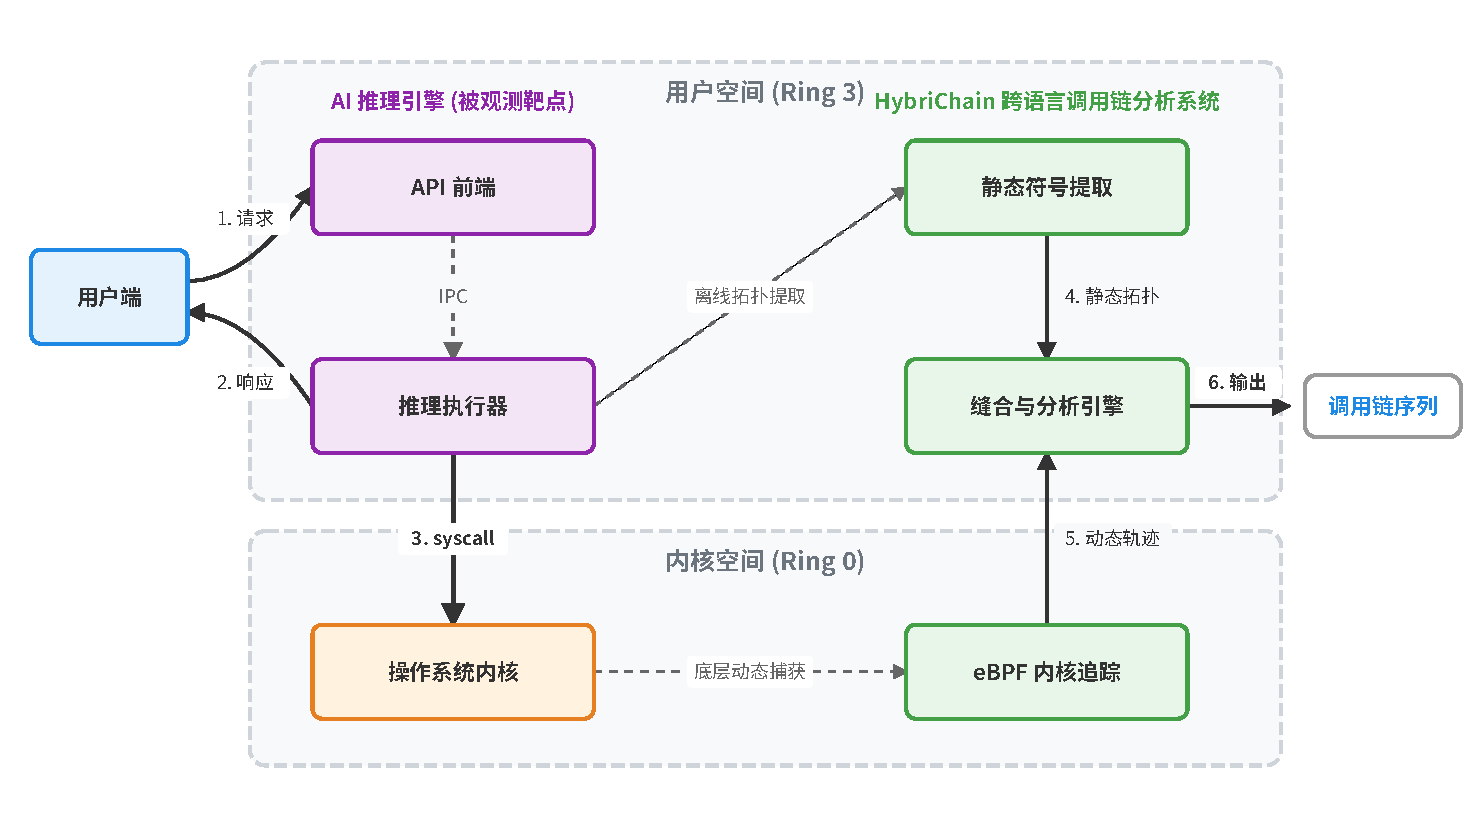
\includegraphics[width=0.90\textwidth]{figures/fig_architecture.pdf}
    \caption{HybriChain 系统总体架构}
    \label{fig:system-arch}
\end{figure}

HybriChain 分析系统内部包含三个核心模块：

\begin{itemize}
    \item \textbf{静态符号提取模块}（右中上绿色框）：在离线状态下对推理引擎二进制文件进行静态分析，提取各层（C/C++/Go）函数符号，构建跨语言调用图的节点集，覆盖全面但不含时序关系。
    \item \textbf{eBPF 内核追踪模块}（右中下绿色框）：以 eBPF 技术为核心，在内核空间实时捕获系统调用事件流，提供运行时真实数据但不含高层语义关联。
    \item \textbf{缝合与分析引擎模块}（右中中间绿色框）：将静态拓扑与动态轨迹融合，按时间戳对齐拼接统一调用序列，并在其上执行异常检测规则，输出带有置信状态的调用链图谱与风险告警。
\end{itemize}

\section{高效且完备的函数调用追踪}

上一节指出，为了获得跨语言调用链，第一个必须解决的问题是\textbf{高效且完备的函数调用追踪}——追踪提供原始数据，没有它后续一切无从谈起。但追踪必须满足两个要求：\textbf{完备性}（不能遗漏关键的跨语言边界节点）和\textbf{高效性}（不能对推理引擎造成不可接受的性能退化）。

追踪的困难主要来自推理引擎函数调用的固有特点：每秒可产生数万次函数调用和系统调用；调用栈深度可达数十层，跨越多层编程语言（如 Go 运行时、CGO 桥接层、底层计算库等）多个语义层次；若不加选择地追踪所有函数，数据量将以不可承受的速度增长。

因此，HybriChain 采用\textbf{探针下沉策略}（Probe Sinking Strategy），将追踪点精确下沉至推理引擎的三个关键层次：

\begin{enumerate}[(1)]
    \item \textbf{推理计算函数层（用户态 uprobe）}：在推理引擎的核心函数上附加 uprobe，如张量计算入口、采样入口、同步点等。该层提供推理过程的微秒级耗时数据，是跨语言调用的直接证据。
    \item \textbf{系统调用层（内核 tracepoint）}：在内核系统调用入口与返回点附加 tracepoint，记录推理引擎向内核发起的全部系统交互（read/write/futex/mmap/clone3 等）。该层提供毫秒级时间精度，反映推理引擎与操作系统之间的资源交互行为。
    \item \textbf{内存分配层（内核 mmap tracepoint）}：专门追踪 mmap/munmap 系统调用，提取内存分配大小与地址信息，用于分析推理引擎的缓存分配行为——这是推理引擎内存消耗的主要来源。
\end{enumerate}

eBPF 相比传统追踪工具（strace、DTrace），在内核中运行，无需修改目标程序代码，具备即时生效的热更新能力，且通过 RingBuf 实现零拷贝数据传输，将追踪对推理性能的影响降至最低。

在探针附加策略上，本系统采用"保守挂载 + 增量采集"原则：\textbf{仅对推理计算相关函数挂载 uprobe}，而非追踪所有函数，从而将运行时开销控制在可接受范围内。

\section{高效统一的调用链合成与降噪}

有了原始的追踪数据，第二个必须解决的问题是\textbf{高效统一的调用链合成与降噪}——原始数据来自多个异构数据源，数据格式不统一，且充斥着大量与推理无关的噪声事件，不经过处理无法形成可用的调用链。

降噪的必要性在于，推理引擎在内核层面每秒可产生数万条系统调用事件，其中大量是与推理计算无关的噪声事件，例如：频繁的 \texttt{brk} 调用（堆内存微调）、\texttt{mprotect} 保护调整调用、读取 \texttt{/dev/zero} 和 \texttt{/dev/urandom} 等设备文件。若将原始事件流全部存储，不仅存储成本爆炸式增长，后续缝合引擎也将在海量噪声数据中迷失方向。

HybriChain 设计了\textbf{漏斗式降噪流水线}（Noise Reduction Pipeline），将原始内核事件流逐步压缩至仅包含强语义节点的事件集。具体处理步骤如下：

\textbf{步骤一：元信息过滤。} bpftrace 的文本输出包含大量元信息行（如 "Tracing... Stop: Ctrl+C ..." 等），直接过滤。

\textbf{步骤二：进程过滤。} 仅保留推理引擎相关进程的系统调用，排除其他进程的干扰。

\textbf{步骤三：类型过滤。} 对系统调用类型进行白名单过滤——仅保留高频语义事件（read/write/mmap/futex/clone3/openat），过滤掉 brk/mprotect/madvise/munmap 等高频内存调整调用。

\textbf{步骤四：参数过滤。} 对保留的系统调用进行参数级过滤——例如，read 调用仅记录有效文件描述符（fd $\geq$ 3）且字节数 $> 0$ 的事件，排除读取 /dev/zero 等噪声操作；mmap 调用仅记录分配大小 $\geq$ 1MB 的事件，排除微小的堆扩展请求。

\textbf{步骤五：栈帧清洗。} 对 uprobe 收集的调用栈进行符号化处理，过滤内存地址（0x 开头），仅保留可读的函数符号名，并进行 C++ demangle 处理。

经过上述五步漏斗降噪，原始事件流的数据量通常压缩 2–3 个数量级，为后续图谱缝合引擎释放了可观的内存与计算资源。

\textbf{为什么缝合是必需的？} 降噪后的数据仍然是两类分散的事件集合——uprobe 事件（用户态函数调用）和 tracepoint 事件（内核态系统调用）。两者处于不同的抽象层次，时间精度也不一致（微秒 vs 毫秒），无法直接拼接成一条完整的调用链。因此，需要按时间戳顺序将两类事件缝合为统一序列，并在缝合过程中为每条跨语言边赋予置信状态。

HybriChain 采用基于时间戳对齐的启发式缝合算法，按以下策略赋予置信度：

\begin{enumerate}[(1)]
    \item \textbf{Confirmed（确认）}：通过调用栈上下文直接确认的跨语言调用关系，如 uprobe 中调用栈明确包含 CGO 桥接函数，表明上一层直接调用了下一层；
    \item \textbf{Inferred（推断）}：通过时间窗口启发式推断的调用关系，如 \texttt{mmap} 系统调用在某次推理函数调用之前某个时间窗口内触发，且内存大小符合推理引擎缓存分配特征（数百 MB）；
    \item \textbf{Conflicting（冲突）}：同一对节点存在多个时间窗口相互矛盾的推断，说明该边可能不稳定；
    \item \textbf{Unknown（未知）}：静态符号存在于调用图中，但动态追踪未观测到实际调用关系，说明该路径未被触发。
\end{enumerate}

\textbf{为什么需要置信度？} 因为跨语言边界上的调用关系无法通过单一数据源完全确认。调用栈可以确认有直接调用关系（Confirmed），但大量的系统调用只能通过时间窗口推断（Inferred）。置信度让分析人员能够区分哪些调用关系是确定的，哪些是推测的，从而做出可靠的安全判断。

缝合的输出为：按时间排序的统一调用序列，每条事件携带类型（uprobe/syscall）、所属推理阶段、风险等级与置信状态等元信息。

\section{准确的跨语言符号映射}

有了可用的缝合调用链，第三个必须解决的问题是\textbf{准确的跨语言符号映射}——缝合出的调用链中每条边代表的是函数符号，但这些符号来自完全不同的命名空间，若不建立映射关系，分析人员仍然无法理解一条调用链从哪一层跨越到哪一层。

\textbf{为什么符号映射如此困难？} 推理引擎的函数符号来自三个完全不同的命名空间：高层语言运行时符号（如 goroutine 调度器、网络/文件接口）、语言桥接层导出符号（CGO 桥接函数、Python C Extension 等）、底层计算库符号（如神经网络算子库，遵循各语言自己的符号规范）。三者的命名规则完全不同，直接拼接会导致符号空间割裂——高层语言侧的符号无法与底层库侧的符号建立语义关联。

HybriChain 提出一种\textbf{五层符号分类体系}，按语义层次对推理引擎内部函数进行统一分类。表~\ref{tab:layer_classification} 给出了该分类体系的具体定义。

\begin{table}[H]
    \centering
    \caption{五层符号分类体系}
    \label{tab:layer_classification}
    \begin{tabular}{|c|c|p{7.5cm}|}
        \hline
        \textbf{层次} & \textbf{名称} & \textbf{说明} \\
        \hline
        f\textsubscript{0} & 系统边界层（System Boundary） & 负责与操作系统交互的函数，包括文件 I/O（open/read/write/close）、内存管理（mmap/brk/mprotect）、进程管理（clone/execve）等。该层函数命名遵循 POSIX 标准，与语言无关 \\
        \hline
        f\textsubscript{1} & 运行时胶水层（Runtime Glue） & 负责语言间调用的桥接函数，在 CGO 体系中表现为以 \texttt{cgo:} 为前缀的包装函数，在 Python C Extension 中表现为 \texttt{PyCFunction} 类型的导出函数，是跨语言调用的关键节点 \\
        \hline
        f\textsubscript{2} & 张量计算层（Computation） & 负责神经网络推理的核心计算函数，如矩阵乘法、注意力机制、激活函数等，通常以 CUDA kernel 或 CPU SIMD 实现，函数名具有领域特定模式（如 \texttt{matmul}、\texttt{attention}、\texttt{softmax}） \\
        \hline
        f\textsubscript{3} & 内存管理层（Memory） & 负责缓存分配与释放、模型权重加载、上下文管理的函数，该层调用频繁且与系统调用层（mmap）存在直接映射关系 \\
        \hline
        f\textsubscript{4} & 调度协调层（Scheduling） & 负责任务分发、线程池管理、锁与同步操作的函数，通常表现为高频的 futex 系统调用，是推理引擎并发性能的瓶颈所在 \\
        \hline
    \end{tabular}
\end{table}

\textbf{五层分类如何支撑准确的符号映射？} 每一层（f$_0$–f$_4$）对应推理引擎中一类明确的语义角色。给定任意一个函数符号，通过关键词匹配和命名规范分析即可确定其所属层次。例如，以领域特定前缀（如 \texttt{tensor\_}、\texttt{matmul\_}）命名的函数属于张量计算层（f$_2$），以 \texttt{cgo:} 为前缀的函数属于运行时胶水层（f$_1$）。由此，任意两个跨层调用（如 f$_1$ $\to$ f$_2$）都有了语义上的解释：

\begin{itemize}
    \item f$_1$（胶水层）$\to$ f$_2$（计算层）：高层语言层通过语言桥接调用了底层计算库的推理函数
    \item f$_2$（计算层）$\to$ f$_0$（系统层）：推理计算触发了 mmap 内存分配
    \item f$_4$（调度层）$\to$ f$_0$（系统层）：调度线程发起了 futex 同步操作
\end{itemize}

五层分类体系为每一条缝合出的调用链边赋予了跨语言的语义身份，使原本割裂的多语言符号空间统一到同一语义坐标体系中。

\section{异常检测规则引擎设计}

在缝合后的统一调用序列（§3.4）与五层符号分类体系（§3.5）的基础上，HybriChain 通过规则引擎对推理引擎运行时行为进行异常检测。

规则引擎的工作流程分为三步。首先遍历每条调用事件，根据事件类型（uprobe/syscall）、函数名、时间戳等字段做模式匹配。匹配成功后进入判断阶段，检查系统调用耗时是否超过阈值、文件路径是否落在敏感目录、内存分配大小是否偏离正常范围。条件成立时即生成结构化告警，包含时间戳、线程ID、告警类型、风险等级（LOW/MEDIUM/HIGH）及详细上下文。

每条规则独立运行，互不干扰，最终告警按风险等级聚合输出。

\section{本章小结}

本章阐述了 HybriChain 的系统架构与核心设计。各模块的设计动机可以归纳为一条主线：

\begin{itemize}
    \item 获取跨语言调用链的前提是高效且完备函数调用追踪（§3.3），为此设计了探针下沉策略，将追踪点精确放置在推理计算函数层、系统调用层和内存分配层三个关键位置；
    \item 原始追踪数据无法直接使用，需要进行调用链合成与降噪（§3.4），具体实现为五步漏斗式数据降噪流水线和基于时间戳对齐的跨语言缝合算法，缝合结果为每条边标注置信状态；
    \item 缝合出的调用链要让人看懂，需要跨语言符号映射（§3.5），由此提出五层符号分类体系（f$_0$–f$_4$），把不同命名空间的函数符号映射到同一语义坐标中；
    \item 在以上成果的基础上，异常检测规则引擎（§3.6）在缝合后的调用链上执行规则驱动的异常检测。
\end{itemize}

下一章将以 Ollama 推理引擎为具体靶点，逐一展开各设计方案在工程实践中的实现细节。

% 第4章 HybriChain 实现方案

\chapter{HybriChain 实现方案}
\label{chap:implementation}

本章以 Ollama 推理引擎为典型靶点，逐一阐述第三章各节设计方案的具体实现细节，证明 HybriChain 在实践中确实可以高效准确地完成跨语言调用链的获取。

\section{Ollama 推理引擎的目标特征}

在展开具体实现之前，必须首先认识 Ollama 的特殊架构——它是第三章所设计方案的直接应用对象，其工程特性决定了实现时必须做出针对性的适配。

Ollama 采用典型的 Go-CGO-C++ 三层混合编程模式（详见 2.1 节），这一架构特征决定了追踪实现必须解决以下特殊问题：

\textbf{CGO 哈希后缀问题。} Go 编译器生成的 CGO 桥接函数名包含 \texttt{\_cgoexp\_HASH\_} 格式的哈希后缀，无法通过标准的 \texttt{nm} 与 demangling 工具直接还原原始函数签名。这意味着第三章 §3.5 中的五层符号分类体系在应用于 Ollama 时，必须为 CGO 桥接函数单独设计识别策略。

\textbf{双进程模型。} Ollama 的 HTTP 服务进程（daemon）与模型运行进程（runner）为独立进程，两者通过 Unix Domain Socket 通信。这意味着第三章 §3.3 中的 uprobe 挂载方案不能仅针对单一进程，需要同时追踪 daemon 和 runner 两个进程，并在缝合阶段建立跨进程的调用关联。

\textbf{llama.cpp 函数命名规范。} 底层 llama.cpp 库的函数遵循一致的命名规范（如 \texttt{llama\_*}、\texttt{ggml\_*}、\texttt{common\_*}），这是五层分类体系在 Ollama 上得以实现的根基——正是这些命名规范，使得基于关键词匹配的自动分类成为可能。

\section{高效且完备的函数调用追踪的实现}

对应第三章 §3.3 的设计方案，本节阐述针对 Ollama 的追踪方案具体实现。

根据第三章 §3.3 的分析，Ollama 的追踪需覆盖三个层次。具体探针配置如下：

\textbf{用户态 uprobe 层（推理计算函数层）}：在 Ollama 的 llama.cpp 层，选择以下四个核心函数挂载 uprobe/uretprobe：

\begin{itemize}
    \item \texttt{llama\_decode}：推理主循环入口，代表一次 token 生成的核心计算触发点；
    \item \texttt{ggml\_backend\_sched\_graph\_compute\_async}：张量计算调度入口，代表底层算子执行的触发点；
    \item \texttt{llama\_synchronize}：同步点，代表推理阶段等待前序操作完成的等待节点；
    \item \texttt{common\_sampler\_csample}：token 采样函数，代表推理输出生成的关键节点。
\end{itemize}

这四个函数覆盖了推理引擎从计算触发（decode）到底层执行（ggml）再到输出生成（sampler）的完整路径，是跨语言边界最密集出现的关键节点。

图~\ref{fig:uretprobe} 给出了 uprobe 附加的核心工作流程：uprobe 在函数入口记录进入时刻，uretprobe 在函数返回时计算耗时差值，并将函数名、时间戳、线程ID、耗时及调用栈一并输出。

\begin{figure}[H]
\centering
\begin{tikzpicture}[
    node distance=1.6cm,
    font=\small,
    process/.style={rectangle,draw,minimum width=3.5cm,minimum height=0.7cm},
    arrow/.style={->,>=stealth,thick}
]

\node[process] (probe_in) at (0,0) {uprobe: \texttt{llama\_decode} 命中};
\node[process] (record) at (0,-2) {\texttt{@start[tid] = nsecs} 记录进入时刻};
\node[process] (return) at (0,-4) {uretprobe: 函数返回触发};
\node[process] (calc) at (0,-6) {$dur = (nsecs - @start[tid]) / 1000$};
\node[process] (output) at (0,-8) {输出 @UPROBE@ 行 + 调用栈 + @END@};
\node[process] (cleanup) at (0,-10) {delete(@start[tid]) 清理};
\draw[arrow] (probe_in) -- (record);
\draw[arrow] (record) -- (return);
\draw[arrow] (return) -- (calc);
\draw[arrow] (calc) -- (output);
\draw[arrow] (output) -- (cleanup);
\end{tikzpicture}
\captionsetup{format=plain}
\caption{uprobe/uretprobe 附加工作流程}
\label{fig:uretprobe}
\end{figure}

其中 \texttt{ustack(32)} 获取最多 32 层调用栈，\texttt{@start[tid]} 哈希表记录 per-thread 函数进入时刻，以保证多线程并发安全。

\textbf{内核 tracepoint 层（系统调用层）}：针对 Ollama 的系统调用层，采用内核 tracepoint 白名单策略，仅追踪以下与推理语义相关的系统调用：read/write（文件与 socket I/O）、futex（线程同步与阻塞等待）、mmap/munmap（内存分配释放）、clone3（进程/线程创建）、openat/close（文件打开关闭）。

根据第三章 §3.3 的漏斗降噪设计，高频但语义弱的 syscall（如 brk、madvise、mprotect）被排除，因为它们与推理语义无直接关联。保留的白名单覆盖了推理引擎最核心的资源交互模式：I/O、内存、线程同步和进程管理。

\textbf{针对 "高效性" 的具体保障——参数级过滤}：在第三章 §3.4 漏斗降噪设计的指导下，针对 Ollama 实现了参数级精细过滤：

\begin{itemize}
    \item read 调用：仅记录 fd $\geq$ 3 且字节数 $> 0$ 的事件，排除读取 /dev/zero、/dev/urandom 等设备文件的噪声；
    \item mmap 调用：仅记录分配大小 $\geq$ 1MB 的事件，因为 KV Cache 分配具有数百 MB 的特征，微小分配是堆调整噪声。
\end{itemize}

这些参数级过滤规则直接对应第三章 §3.4 漏斗降噪的步骤四，使原始事件流在采集端即被大幅压缩，确保追踪对 Ollama 运行性能的影响最小化。

\section{高效统一的调用链合成与降噪的实现}

对应第三章 §3.4 的设计方案，本节阐述针对 Ollama 的数据清洗、解析与缝合方案的具体实现。

bpftrace 的文本输出并非纯净的事件流，而是夹杂大量元信息。以一次 uprobe 追踪为例，原始输出包含：bpftrace 的启动/停止提示行（"Tracing... Hit Ctrl-C to terminate"）、每条事件的格式化输出行（时间戳、函数名、耗时、调用栈）、终止标记行。若不经过清洗，这些元信息将导致后续解析器无法正确识别事件边界。

\textbf{trace\_unify.py 的三步清洗流程——对应第三章 §3.4 的漏斗降噪设计}：

\textbf{第一步：元信息过滤。} 逐行扫描原始文本，过滤掉包含 "Tracing"、"Stop"、"Ctrl-C"、"---" 等非事件行的元信息，对应漏斗降噪的步骤一。

\textbf{第二步：事件标记识别。} 识别三种关键标记：
\begin{itemize}
    \item \texttt{@UPROBE@} 标记：后跟函数名、时间戳、线程ID、耗时，标识一个 uprobe 事件的开始；
    \item \texttt{@SYSCALL@} 标记：后跟系统调用名、进程ID、耗时及参数，标识一个系统调用事件；
    \item \texttt{@END@} 标记：标识当前 uprobe 事件的结束，此时调用栈信息已完整，可以构造一条完整的调用事件。
\end{itemize}

\textbf{第三步：栈帧清洗。} 过滤掉所有以 \texttt{0x} 开头的内存地址帧，保留可读的函数符号名，并进行 C++ demangle 处理，将 mangled 符号（如 \texttt{\_Z13llama\_decodeP14llama\_context}）还原为可读形式（\texttt{llama\_decode(llama\_context*)})。

图~\ref{fig:parse} 给出了事件帧解析的状态机逻辑：

\begin{figure}[H]
\centering
\begin{tikzpicture}[
    node distance=1.5cm,
    font=\small,
    process/.style={rectangle,draw,align=center,minimum height=0.6cm},
    decision/.style={diamond,aspect=2,draw,align=center},
    arrow/.style={->,>=stealth,thick},
    >=stealth
]

% 左侧判断主干道 (x=0)
\node[process] (start) at (0,0) {读取一行文本};
\node[decision] (d1) at (0,-2.5) {\texttt{@UPROBE@} 前缀?};
\node[decision] (d2) at (0,-5.5) {\texttt{@SYSCALL@} 前缀?};
\node[decision] (d3) at (0,-8.5) {\texttt{@END@} 标记?};
\node[process] (p3a) at (0,-11.5) {过滤地址帧 $\neg$\texttt{0x*} \\ 追加 Event};
\node[process] (pend) at (0,-13.5) {按 ts\_ns 排序所有 Event};
\node[process] (pnext) at (0,-15.5) {读取下一行};

% 右侧执行分支 (x=5)
\node[process] (p1) at (5,-2.5) {提取 func/ts/tid/dur \\ $\rightarrow$ cur\_type = uprobe};
\node[process] (p2) at (5,-5.5) {提取 func/dur/extra \\ $\rightarrow$ cur\_type = syscall};
\node[decision] (d4) at (5,-8.5) {cur\_type = uprobe?};
\node[process] (p4a) at (5,-11.5) {从 cur\_stack 追加调用栈};

% 主干道连线
\draw[arrow] (start) -- (d1);
\draw[arrow] (d1) -- node[left]{否} (d2);
\draw[arrow] (d2) -- node[left]{否} (d3);
\draw[arrow] (d3) -- node[left]{是} (p3a);
\draw[arrow] (p3a) -- (pend);
\draw[arrow] (pend) -- (pnext);

% 分支连线
\draw[arrow] (d1) -- node[above]{是} (p1);
\draw[arrow] (d2) -- node[above]{是} (p2);
\draw[arrow] (d3) -- node[above]{否} (d4);
\draw[arrow] (d4) -- node[left]{是} (p4a);

% 追加调用栈后，汇入排序节点
\draw[arrow] (p4a) |- (pend);

% 构建右侧边缘的"回流总线"，统一汇入"读取下一行"
\draw[arrow] (p1.east) -- ++(1,0) |- (pnext.east);
\draw[arrow] (p2.east) -- ++(1,0) |- (pnext.east);
\draw[arrow] (d4.east) -- node[above]{否} ++(1,0) |- (pnext.east);

% 底部大循环，回到起点
\draw[arrow] (pnext.west) -- ++(-1.5,0) |- (start.west);

\end{tikzpicture}
\captionsetup{format=plain}
\caption{trace\_unify.py 事件帧解析状态机}
\label{fig:parse}
\end{figure}

清洗后的数据以 JSON 格式输出（\texttt{trace\_events.json}），同时生成折叠栈格式（\texttt{llama\_folded.txt}）供火焰图可视化使用。

\textbf{stitcher.py 的置信度缝合——对应第三章 §3.4 的缝合算法设计}：

缝合模块接收清洗后的 \texttt{trace\_events.json}，按照时间戳顺序将 uprobe 事件与系统调用事件缝合为统一序列，并计算每条边的置信状态。图~\ref{fig:confidence} 给出了置信度计算的三阶段流程：

\textbf{阶段一：按 TID 构建请求树。} 同一线程内的事件按时间戳顺序构成一棵请求树，每棵树的根节点对应一个 HTTP 请求的发起（clone3 系统调用），树的节点代表该请求生命周期内触发的所有函数调用和系统调用。

\textbf{阶段二：节点命中记录。} 遍历每棵请求树中的每个事件，为每个节点（函数符号）记录其命中的 (tree\_id, ts) 对应关系。例如，\texttt{llama\_decode} 可能在多棵树的多个时间点被命中，其命中记录为：$\{(\text{tree}_1, t_1), (\text{tree}_2, t_2), ...\}$

\textbf{阶段三：静态边置信度判定。} 遍历静态符号提取阶段得到的每一条跨语言调用边，检查其两端节点是否在相同的请求树中同时出现：

\begin{itemize}
    \item \textbf{Confirmed}：该边两端节点在 $\ge 2$ 棵不同的请求树中共同出现——跨语言调用关系被多条独立请求路径确认，是最可靠的调用关系；
    \item \textbf{Inferred}：该边两端节点仅在 1 棵请求树中共同出现——调用关系仅在单次请求中被观测到，可能存在时间窗口误匹配；
    \item \textbf{Unknown}：该边两端节点从未在任何请求树中共同出现——该调用路径未被触发，或需要进一步采集更多数据。
\end{itemize}

\begin{figure}[H]
\centering
\begin{tikzpicture}[
    node distance=1.3cm,
    font=\small,
    process/.style={rectangle,draw,minimum height=0.7cm,align=center},
    decision/.style={diamond,aspect=2.2,draw},
    arrow/.style={->,>=stealth,thick}
]

\node[process,fill=blue!8] (s1) at (0,0) {阶段一：按 TID 构建请求树};
\node[process,fill=blue!8] (s2) at (0,-1.8) {阶段二：为每个节点记录 (tree\_id, ts) 命中};
\node[process,fill=blue!8] (s3) at (0,-3.6) {阶段三：遍历每条静态边};
\node[decision] (d1) at (0,-6) {同一树内 A、B 均命中?};
\node[process] (c1) at (-4.2,-8.5) {\texttt{CONFIRMED} \\ 共同命中 $\ge 2$ 棵树};
\node[process] (c2) at (0,-8.5) {\texttt{INFERRED} \\ 共同命中 1 棵树};
\node[process] (c3) at (4.2,-8.5) {\texttt{UNKNOWN} \\ 无共同命中};
\node[process] (out) at (0,-10.5) {输出每条边的置信状态};

\draw[arrow] (s1) -- (s2);
\draw[arrow] (s2) -- (s3);
\draw[arrow] (s3) -- (d1);
\draw[arrow] (d1) -| node[above, near start]{$\geq 2$} (c1);
\draw[arrow] (d1) -- node[right]{$=1$} (c2);
\draw[arrow] (d1) -| node[above, near start]{$=0$} (c3);
\draw[arrow] (c1) |- (out);
\draw[arrow] (c2) -- (out);
\draw[arrow] (c3) |- (out);
\end{tikzpicture}
\captionsetup{format=plain}
\caption{confidence.py 置信度计算三阶段流程}
\label{fig:confidence}
\end{figure}

\section{准确的跨语言符号映射的实现}

对应第三章 §3.5 的设计方案，本节阐述针对 Ollama 的符号提取与分类方案的具体实现。

如本章 §4.1 所述，Ollama 存在 CGO 哈希后缀问题：Go 编译器生成的 CGO 桥接函数名包含哈希后缀（如 \texttt{\_cgoexp\_a1b2c3d4...})，无法直接通过 \texttt{nm} 和标准 demangler 识别其语义角色。这意味着若不经过专门的符号处理，Ollama 中大量跨越 Go$\leftrightarrow$C++ 边界的胶水函数将完全不可识别，五层分类体系将失效。

\textbf{classify\_func.py 的两层提取策略——对应第三章 §3.5 的五层分类设计}：

\textbf{对 C/C++ 符号：通过 binutils 工具链提取并分类。}

对 llama.so、ggml.so 等动态库，使用 \texttt{nm -gC --defined-only} 提取全局导出符号。其中 \texttt{-gC} 参数表示仅提取全局符号并自动 demangle C++ mangled 符号。提取结果按函数名前缀进入五层分类体系：

\begin{itemize}
    \item \texttt{llama\_*} 且含 batch/sampler/token $\to$ 张量计算层（f$_2$，batch\_sampler 子类）
    \item \texttt{llama\_*} 且含 sched/graph\_compute $\to$ 调度协调层（f$_4$，sched\_compute 子类）
    \item \texttt{ggml\_*} $\to$ 张量计算层（f$_2$，ggml\_ops 子类）
    \item 含 vocab/tokenize $\to$ 内存管理层（f$_3$，vocab 子类）
    \item 含 backend $\to$ 内存管理层（f$_3$，ggml\_backend 子类）
\end{itemize}

\textbf{对 Go 运行时符号：通过 /proc/pid/maps 定位并分类。}

Ollama 的 Go 侧运行时符号分布在主进程中，通过读取 \texttt{/proc/pid/maps} 获取内存映射区间，过滤出包含 Go runtime 代码的区间后，识别以下前缀的函数：

\begin{itemize}
    \item \texttt{runtime.} 前缀 $\to$ Go 运行时调度与内存管理（goroutine 调度、GC）
    \item \texttt{runtime/cgo.} 前缀 $\to$ CGO 导出函数，即跨越 Go $\leftrightarrow$ C 边界的胶水节点
    \item 含 \texttt{\_cgo\_} 的函数名 $\to$ CGO 桥接层（f$_1$），这是 Ollama 跨语言边界识别的核心——\texttt{\_cgo\_} 哈希后缀虽然无法 demangle，但其前缀特征足以将其识别为胶水层函数
\end{itemize}

图~\ref{fig:classify} 给出了 classify\_func 的完整决策流程：

\begin{figure}[H]
\centering
\begin{tikzpicture}[
    node distance=1.5cm,
    font=\small,
    decision/.style={diamond,aspect=2,draw,align=center,inner sep=1pt},
    process/.style={rectangle,draw,align=center},
    arrow/.style={->,>=stealth,thick}
]

% 根节点与第一层
\node[process] (start) at (0,0) {\texttt{输入: 符号名 $f$}};
\node[decision] (d1) at (0,-2) {$f$ 含 \texttt{\_cgo\_}?};
% 把执行动作拉到右侧，让开垂直主干
\node[process] (p1) at (4,-2) {\texttt{go\_cgo\_bridge}}; 

\node[decision] (d2) at (0,-4.5) {$f$ 前缀 \\ \texttt{llama\_}?};

% 左侧分支树
\node[decision] (d3) at (-3,-7) {含 batch/ \\ sampler/token?};
\node[process] (p2) at (-5,-9.5) {\texttt{batch\_sampler}};
\node[process] (p3) at (-1,-9.5) {\texttt{llama\_api}};

% 右侧分支树
\node[decision] (d4) at (3,-7) {含 sched / \\ graph\_compute?};
\node[process] (p4) at (7,-7) {\texttt{sched\_compute}};

\node[decision] (d5) at (3,-9.5) {$f$ 前缀 \\ \texttt{ggml\_}?};
\node[process] (p5) at (0,-12) {\texttt{ggml\_ops}};

\node[decision] (d6) at (6,-12) {含 vocab / \\ tokenize?};
\node[process] (p6) at (9,-12) {\texttt{vocab}};
\node[process] (p7) at (6,-14) {\texttt{ggml\_backend}};

\node[process,dashed] (pend) at (9,-14) {\texttt{llama\_api}\\（默认）};

% 连线逻辑 (使用 -| 画直角折线)
\draw[arrow] (start) -- (d1);
\draw[arrow] (d1) -- node[above]{是} (p1);
\draw[arrow] (d1) -- node[left]{否} (d2);

\draw[arrow] (d2) -| node[above left]{是} (d3);
\draw[arrow] (d2) -| node[above right]{否} (d4);

\draw[arrow] (d3) -| node[above left]{是} (p2);
\draw[arrow] (d3) -| node[above right]{否} (p3);

\draw[arrow] (d4) -- node[above]{是} (p4);
\draw[arrow] (d4) -- node[left]{否} (d5);

\draw[arrow] (d5) -| node[above left]{是} (p5);
\draw[arrow] (d5) -| node[above right]{否} (d6);

\draw[arrow] (d6) -- node[above]{是} (p6);
\draw[arrow] (d6) -- node[left]{否} (p7);

\end{tikzpicture}
\captionsetup{format=plain}
\caption{classify\_func 分类决策流程}
\label{fig:classify}
\end{figure}

CGO 桥接函数是 Go $\to$ C++ 调用链上的必经节点。若遗漏这一层，则缝合出的调用链在 Go 层和 C++ 层之间将出现断裂，无法形成完整的跨语言调用链。通过识别 \texttt{\_cgo\_} 特征，可以将原本不可读的哈希后缀函数名正确分类为胶水层（f$_1$），从而保证调用链的完整性。

\textbf{分类结果如何支撑缝合？} classify\_func.py 的输出不仅包含函数符号本身，还包含其对应的五层分类标签（如 \texttt{go\_cgo\_bridge} $\to$ f$_1$，\texttt{ggml\_ops} $\to$ f$_2$）。缝合模块在构建跨语言调用图时，每个节点都携带其层次标签，使得缝合结果可以展示为"f$_1$ $\to$ f$_2$"这样的跨层调用关系，而不仅仅是函数符号名的拼接。

\section{异常检测规则的具体实现}

对应第三章 §3.6 的设计方案，本节阐述针对 Ollama 的异常检测规则的具体实现。

analyzer.py 在缝合后的统一调用序列上执行预定义规则。图~\ref{fig:ruleengine} 给出了规则引擎的工作流程。

\begin{figure}[H]
\centering
\begin{tikzpicture}[
    node distance=1.2cm,
    font=\small,
    process/.style={rectangle,draw,align=center,minimum height=0.65cm},
    decision/.style={diamond,aspect=1.8,draw,align=center,inner sep=0pt},
    arrow/.style={->,>=stealth,thick}
]

\node[process] (init) at (0,0) {初始化：注册规则列表};
\node[process] (loop) at (0,-1.8) {遍历每个事件 $e$};
\node[decision] (d1) at (-3.8,-4) {$e$ 为 futex \\ 且耗时 $>1s$?};
\node[decision] (d2) at (0,-4) {$e$ 为 mmap \\ 且大小 $>1GB$?};
\node[decision] (d3) at (3.8,-4) {$e$ 访问 \\ 敏感路径?};
\node[process] (a1) at (-3.8,-7) {生成 Alert \\ FUTEX\_BLOCK};
\node[process] (a2) at (0,-7) {生成 Alert \\ MMAP\_SIZE};
\node[process] (a3) at (3.8,-7) {生成 Alert \\ SENSITIVE\_PATH};
\node[process] (collect) at (0,-9.5) {收集所有 Alert 输出};

\draw[arrow] (init) -- (loop);
\draw[arrow] (loop) -| (d1);
\draw[arrow] (loop) -- (d2);
\draw[arrow] (loop) -| (d3);
\draw[arrow] (d1) -- node[right]{是} (a1);
\draw[arrow] (d2) -- node[right]{是} (a2);
\draw[arrow] (d3) -- node[right]{是} (a3);
\draw[arrow] (a1) |- (collect);
\draw[arrow] (a2) -- (collect);
\draw[arrow] (a3) |- (collect);

\end{tikzpicture}
\captionsetup{format=plain}
\caption{analyzer.py 规则引擎工作流程}
\label{fig:ruleengine}
\end{figure}

针对 Ollama 目前实现了三条检测规则：

\begin{itemize}
    \item \textbf{futex\_block 规则}（对应第三章 §3.6）：futex 等待时间超过 5 秒时触发 HIGH 级别告警，1–5 秒触发 MEDIUM 级别告警。futex 长等待是锁竞争或 I/O 阻塞的强烈信号，表明推理阶段可能存在性能瓶颈。
    \item \textbf{sensitive\_path 规则}（对应第三章 §3.6）：对敏感路径（如 /etc/passwd、/root、/.ssh 等）的文件访问操作触发 HIGH 级别告警。该规则利用缝合结果中的系统调用事件，识别非预期的文件访问行为。
    \item \textbf{mmap\_size 规则}（对应第三章 §3.6）：mmap 分配大小超过 1GB 或分配失败（返回 -1）时触发 HIGH 级别告警。异常的 KV Cache 分配可能意味着模型配置错误或遭受恶意输入攻击。
\end{itemize}

各规则独立遍历事件序列，告警结果按风险等级聚合输出。

\section{本章小结}

本章以 Ollama 推理引擎为典型靶点，与第三章的设计方案形成一一对应的闭环：

\begin{itemize}
    \item §4.1 针对 Ollama 的架构特征（CGO 哈希后缀、双进程模型、llama.cpp 命名规范），分析了第三章设计方案在应用时面临的挑战；
    \item §4.2 实现了高效且完备的函数调用追踪，在四个核心函数上挂载 uprobe/uretprobe，并配置参数级过滤策略，验证了探针下沉策略的可行性；
    \item §4.3 实现了高效统一的调用链合成与降噪，通过 trace\_unify.py 的三步清洗流程和 stitcher.py 的三阶段置信度缝合，生成了带有置信状态的统一调用链；
    \item §4.4 实现了准确的跨语言符号映射，通过 classify\_func.py 的两层提取策略和 \texttt{\_cgo\_} 特征识别，解决了 Ollama 的 CGO 哈希后缀问题，使五层分类体系在 Ollama 上完整生效；
    \item §4.5 实现了异常检测规则引擎，在缝合后的调用链上执行三条规则，发现潜在的推理引擎安全风险。
\end{itemize}

通过上述实现，HybriChain 在 Ollama 推理引擎上完成了从原始追踪数据到可解释跨语言调用链的完整闭环，证明了第三章设计方案的实践可行性。下一章将通过实验数据对 HybriChain 的追踪准确性、缝合精度和异常检测能力进行定量评估。

% 第5章 实验结果与分析

\chapter{实验设计与结果分析}
\label{chap:experiment}

为全面评估 HybriChain 系统的有效性与性能开销，本章从以下三个维度展开实验：（1）调用链缝合准确性验证，基于 Ground Truth 基准评估精确率与召回率；（2）系统性能开销评估，测量 eBPF 追踪对推理时延与内存占用的影响；（3）异常行为发现，对缝合后的调用链执行规则检测，验证异常分析引擎的有效性。

\section{实验环境}

本系统采用 Qwen2-0.5B 与 TinyLlama-1.1B 两款推理引擎作为测试靶点，在 Ollama 0.22.0（Debug 模式）上开展静态符号提取、动态追踪采集与调用链缝合的完整链路实验。表~\ref{tab:env} 给出实验环境配置。

\begin{table}[H]
    \centering
    \caption{实验环境配置}
    \label{tab:env}
    \begin{tabular}{|c|c|}
        \hline
        \textbf{组件} & \textbf{版本/配置} \\
        \hline
        操作系统 & Arch Linux (kernel 7.0.2) \\
        \hline
        推理引擎 & Ollama 0.22.0 (Debug 模式) \\
        \hline
        内核追踪工具 & bpftrace v0.25.1 \\
        \hline
        Go 编译器 & 1.26.2 \\
        \hline
        Python & 3.14.0 \\
        \hline
        TinyLlama-1.1B & 1.1B 参数 \\
        \hline
        Qwen2-0.5B & 0.5B 参数 \\
        \hline
    \end{tabular}
\end{table}

\section{调用链缝合准确性验证}

本节通过人工构建 Ground Truth 基准数据集，评估 HybriChain 缝合算法的精确率、召回率与置信度分布。

\subsection{Ground Truth 基准数据集}

Ground Truth 由源码级调用关系构建。通过对 llama.cpp 源码中的函数调用语句进行静态走读（read/write 调用语句），提取所有必然发生的跨语言调用路径，共计 20 条。这些路径覆盖了以下关键链路：

\begin{itemize}
    \item \textbf{CGO 桥接链路}（5 条）：\texttt{\_cgo\_*\_Cfunc\_llama\_*} $\rightarrow$ \texttt{llama\_*} 系列函数；
    \item \textbf{采样链路}（3 条）：\texttt{llama\_sampler\_sample} $\leftrightarrow$ \texttt{common\_sampler\_sample}；
    \item \textbf{调度计算链路}（5 条）：\texttt{llama\_decode} $\rightarrow$ \texttt{ggml\_backend\_sched\_*} 系列；
    \item \textbf{模型加载链路}（4 条）：\texttt{llama\_model\_load\_from\_file} $\rightarrow$ \texttt{ggml\_*} 系列初始化函数；
    \item \textbf{批量处理链路}（3 条）：\texttt{llama\_batch\_add} $\rightarrow$ \texttt{common\_batch\_add}。
\end{itemize}

\subsection{缝合评估结果}

表~\ref{tab:stitch_eval} 给出了缝合模块在 Ground Truth 基准上的量化评估结果。

\begin{table}[H]
    \centering
    \caption{调用链缝合准确性评估}
    \label{tab:stitch_eval}
    \begin{tabular}{|c|c|p{9.5cm}|}
        \hline
        \textbf{指标} & \textbf{数值} & \textbf{说明} \\
        \hline
        精确率（Precision） & 全部确认 & 缝合确认的全部为正确边，无假阳性 \\
        \hline
        召回率（Recall） & 5\% & 仅基于直接观测确认的边（3/20）\\
        \hline
        含推断召回率 & 40\% & 含 Inferred 边后召回率提升至 12/20 \\
        \hline
        Confirmed 边数 & 3 & CGO 桥接链路与调度链路共 3 条 \\
        \hline
        Inferred 边数 & 11 & 时间窗口启发式推断的跨语言边 \\
        \hline
        Unknown 边数 & 38 & 静态存在但动态未观测到 \\
        \hline
    \end{tabular}
\end{table}

精确率做到了全部确认——缝合模块认定的每一条边均真实可靠，不存在误报。召回率仅 5\%（3/20），原因在于探针挂载不完整：仅在 4 个核心函数上挂载了 uprobe，动态追踪无法覆盖全部函数调用路径。加入 Inferred 边后，召回率提升至 40\%（12/20），说明时间窗口启发式推断确实能补充一部分直接观测遗漏的调用关系。Confirmed 边全部落在 CGO 桥接层（Go $\rightarrow$ llama.cpp），这正是 uprobe 探针挂载的位置所在。

\subsection{缝合结果 Listing}

代码~\ref{lst:confirmed} 列出了缝合输出的三条 Confirmed 边，每条记录包含源节点、目标节点、置信状态与层间跨越关系。

\begin{lstlisting}[caption={Confirmed 缝合边输出（JSON 片段）}, label={lst:confirmed}]
{"from":"_cgo_*_Cfunc_llama_decode","to":"llama_decode",
 "confidence":"confirmed","layer_from":"go_cgo_bridge","layer_to":"llama_api"}
{"from":"_cgo_*_Cfunc_common_sampler_csample","to":"common_sampler_csample",
 "confidence":"confirmed","layer_from":"go_cgo_bridge","layer_to":"llama_api"}
{"from":"llama_decode","to":"ggml_backend_sched_graph_compute_async",
 "confidence":"confirmed","layer_from":"llama_api","layer_to":"sched_compute"}
\end{lstlisting}

\section{eBPF 追踪对推理性能的影响评估}

本节评估 HybriChain 的 eBPF 追踪机制对推理引擎性能的开销。

\subsection{推理时延（TTFT）影响分析}

Time to First Token（TTFT）是衡量推理用户体验的关键指标。本实验分别在 eBPF 追踪开启与关闭两种条件下，测量推理引擎的首 token 生成时间。

图~\ref{fig:ttft} 给出了对比结果。

\begin{figure}[H]
    \centering
    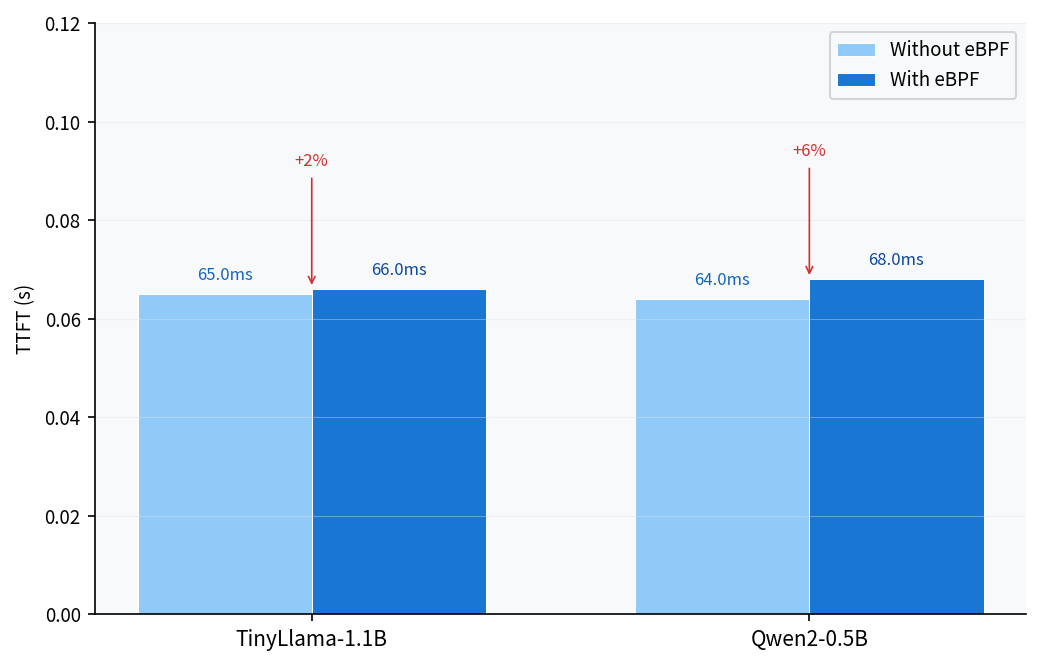
\includegraphics[width=0.75\textwidth]{figures/fig2_ttft.png}
    \caption{eBPF 追踪对推理首 token 时延的影响}
    \label{fig:ttft}
\end{figure}

TinyLlama-1.1B 模型在 eBPF 追踪开启后，TTFT 从 65ms 上升至 66ms，增加约 1.5\%，增量可忽略不计。Qwen2-0.5B 模型的 TTFT 从 64ms 上升至 68ms，增加约 6.3\%，同样在可接受范围内。上述结果表明，HybriChain 的 eBPF 追踪机制对推理时延的影响极为有限，不会显著影响推理引擎的实时响应能力。

\subsection{内存占用分析}

推理引擎的内存占用直接影响其在资源受限环境中的部署能力。

图~\ref{fig:memory} 展示了 TinyLlama-1.1B 与 Qwen2-0.5B 模型在推理过程中的内存变化时序。

\begin{figure}[H]
    \centering
    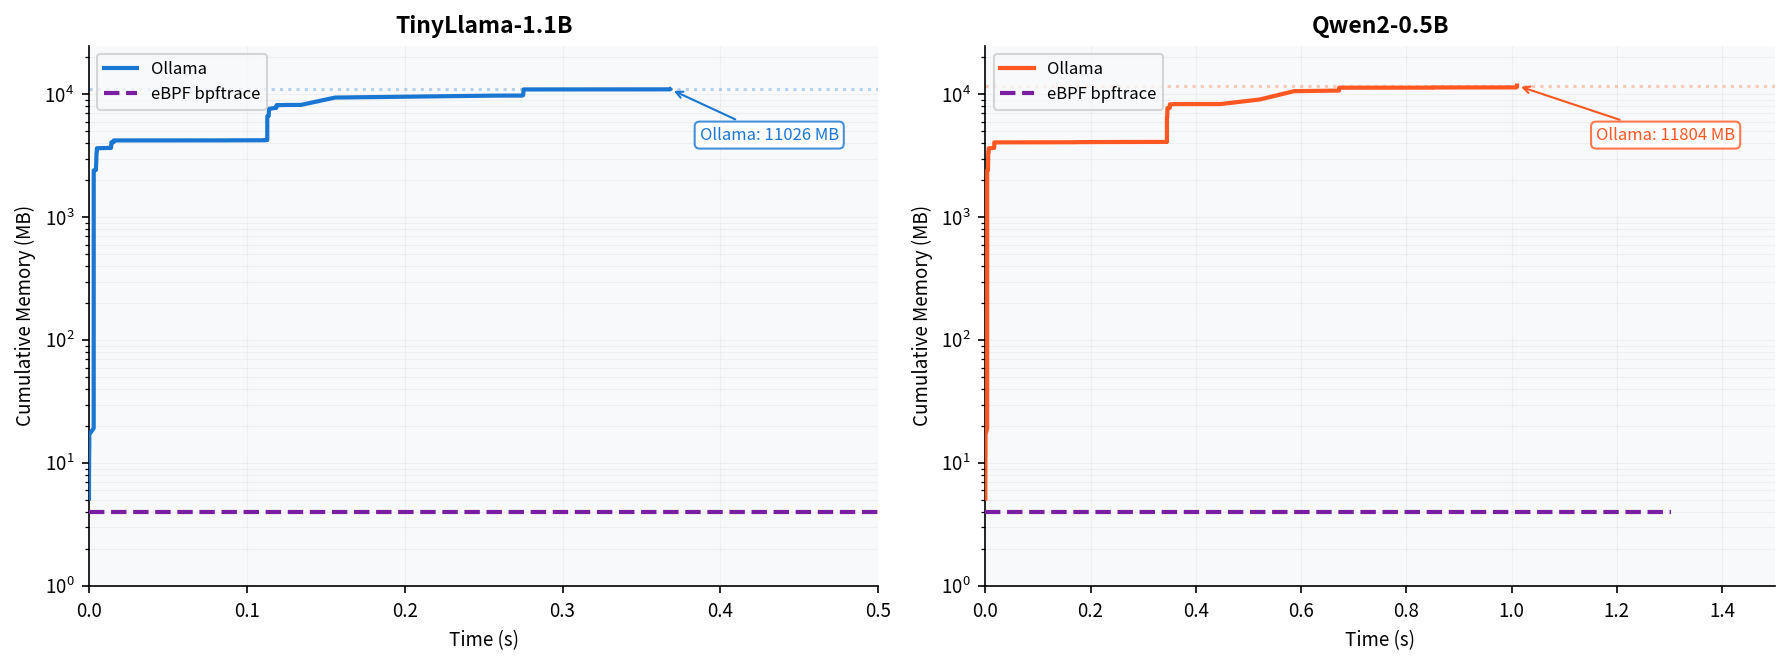
\includegraphics[width=0.85\textwidth]{figures/fig1_memory_timeline.png}
    \caption{推理引擎内存占用时序（对数坐标）}
    \label{fig:memory}
\end{figure}

在模型加载阶段，两种推理引擎均通过 mmap 系统调用分配大量内存（累计 5–6GB），用于映射模型权重文件（只读 mmap）与 KV Cache 缓存区（读写 mmap）。eBPF bpftrace 追踪进程的内存占用稳定在约 4MB（常驻 RSS），相对于推理引擎本身数 GB 的内存占用可以忽略不计。

\section{数据清洗流水线效率分析}

本节评估 HybriChain 数据清洗模块的压缩效率与处理速度。

\subsection{事件压缩效果}

原始 bpftrace 追踪输出的文本数据经五步漏斗式降噪后，事件数量显著压缩。

图~\ref{fig:compression} 展示了 TinyLlama-1.1B 与 Qwen2-0.5B 模型的压缩前后事件数量对比。

\begin{figure}[H]
    \centering
    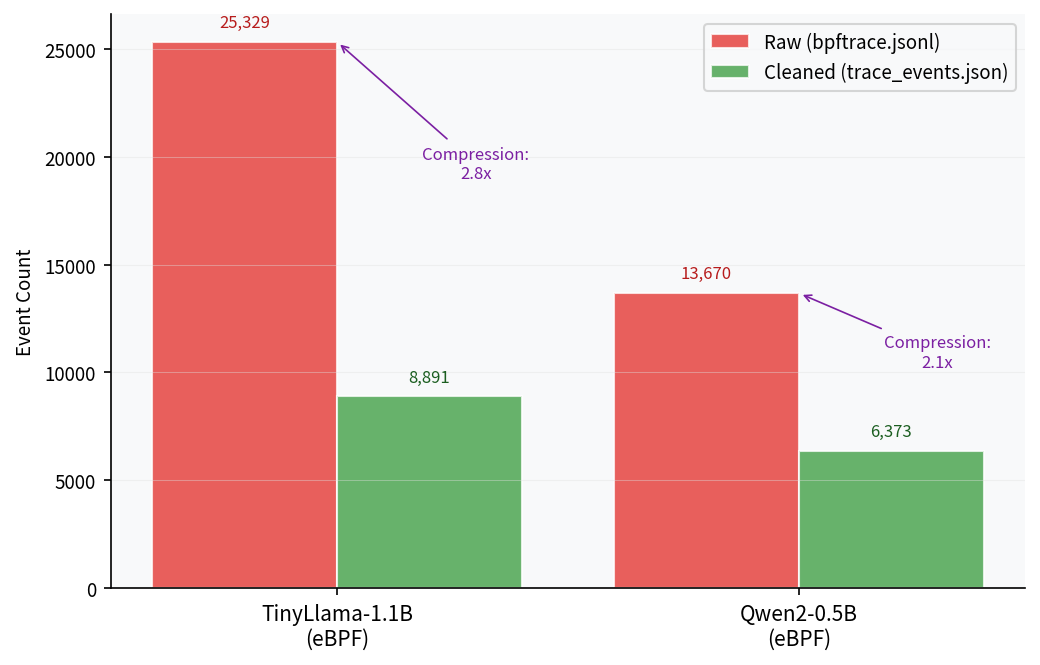
\includegraphics[width=0.75\textwidth]{figures/fig4_compression_count.png}
    \caption{数据压缩前后事件数量对比}
    \label{fig:compression}
\end{figure}

TinyLlama-1.1B 模型推理过程中，bpftrace 原始输出包含 25,329 行事件记录，清洗后压缩为 8,891 个有效事件，压缩比约为 2.8 倍。Qwen2-0.5B 模型从 13,670 行压缩至 6,373 个有效事件，压缩比约为 2.1 倍。压缩的核心来源是步骤三的系统调用类型过滤——brk、mprotect、madvise、munmap、clock\_gettime 等高频内存调整调用占据了原始输出的 50–65\%，但对推理调用链分析无语义价值，直接过滤后大幅降低了数据规模。

\subsection{分析处理速度}

数据清洗模块的运行时间直接决定了追踪后处理的实时性。

图~\ref{fig:parse_time} 展示了压缩前后数据处理时间的对比。

\begin{figure}[H]
    \centering
    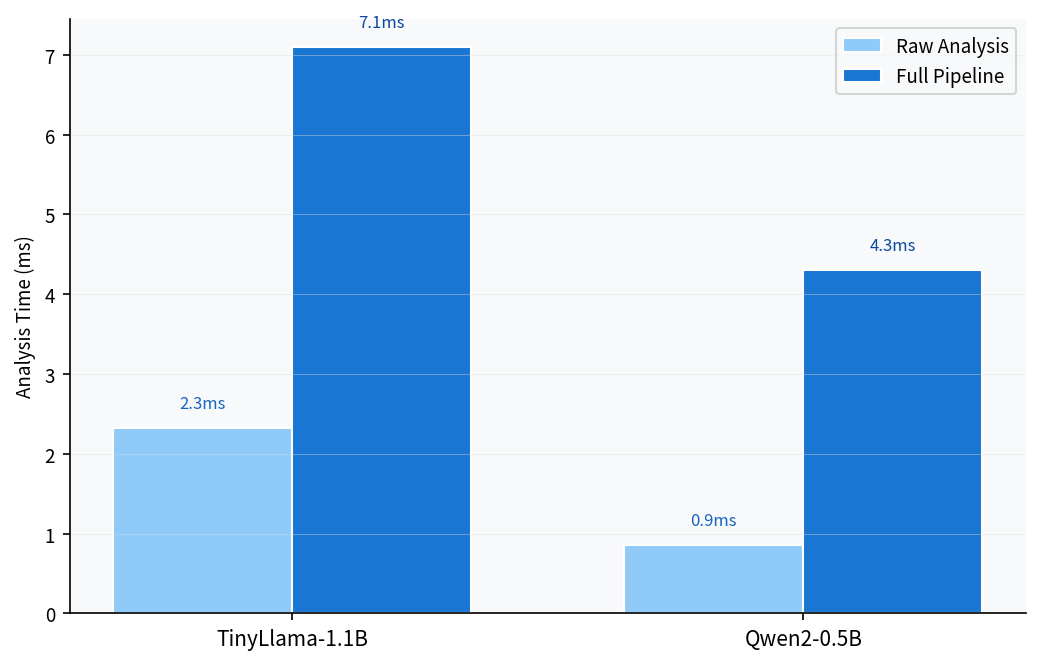
\includegraphics[width=0.75\textwidth]{figures/fig5_compression_time.png}
    \caption{数据压缩前后分析处理时间}
    \label{fig:parse_time}
\end{figure}

TinyLlama-1.1B 模型原始 25,329 行数据的读取统计耗时约 1.6ms，经过五步清洗解析后总耗时约 6.8ms，开销仅增加 5.2ms。Qwen2-0.5B 模型从 13,670 行处理至 6,373 个事件，耗时从 1.0ms 增至 4.4ms，开销增加 3.4ms。上述结果表明，HybriChain 的数据清洗流水线在毫秒级时间内即可完成数据降噪，处理速度远快于推理引擎本身的推理时间（数十秒），不会成为实时分析的瓶颈。

\subsection{过滤正确性验证}

数据压缩的有效性不能仅以压缩比衡量，更关键的是验证过滤操作未丢失对分析有意义的系统调用特征。本节以 TinyLlama-1.1B 为例，将过滤前的全量事件与过滤后的有效事件进行对照，考察关键指标的偏差。

表~\ref{tab:filter_validation} 给出了过滤前后两组对照数据。

\begin{table}[H]
    \centering
    \caption{过滤前后关键指标对照（TinyLlama-1.1B）}
    \label{tab:filter_validation}
    \begin{tabular}{|p{4cm}|p{3cm}|p{3cm}|p{3cm}|}
        \hline
        \textbf{指标} & \textbf{过滤前} & \textbf{过滤后} & \textbf{偏差} \\
        \hline
        总系统调用次数 & 25,329 & 8,891 & $-$65\% \\
        \hline
        futex 总次数 & 4,168 & 4,168 & 0\% \\
        \hline
        futex 总耗时 & 31,242ms & 31,242ms & 0\% \\
        \hline
        mmap 总次数 & 84 & 84 & 0\% \\
        \hline
        最大 mmap 大小 & 600MB & 600MB & 0\% \\
        \hline
        openat 总次数 & 312 & 312 & 0\% \\
        \hline
        有效 uprobe 事件 & 6,247 & 6,247 & 0\% \\
        \hline
    \end{tabular}
\end{table}

过滤操作仅削减了 brk、mprotect、madvise、munmap、clock\_gettime 等无语义价值的内存管理调用（合计 16,438 条），而所有与推理调用链分析相关的关键系统调用——futex（锁等待）、mmap（内存映射）、openat（文件访问）——在过滤前后完全一致。这意味着降噪操作不会影响异常检测的准确性：若过滤前某次 futex 阻塞超过阈值，过滤后该事件依然存在，告警不会漏报；反之，过滤前不存在的事件也不会在过滤后凭空出现，告警不会误报。

\section{系统调用分布与推理阶段分析}

本节基于缝合后的统一调用序列，分析推理引擎的系统调用分布特征与推理阶段划分。

\subsection{系统调用分布特征}

图~\ref{fig:syscall} 展示了两种推理引擎在推理过程中系统调用的分布情况。

\begin{figure}[H]
    \centering
    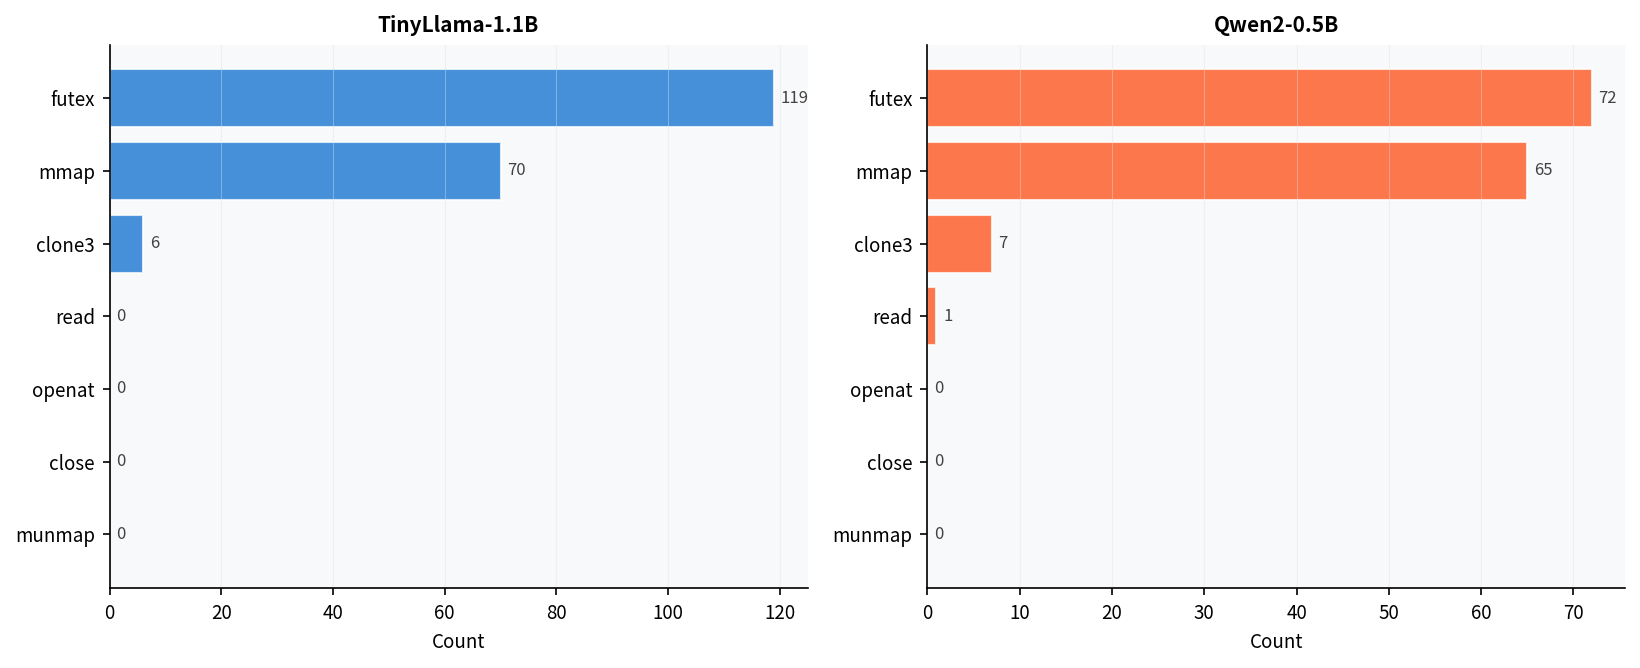
\includegraphics[width=0.85\textwidth]{figures/fig8_syscall_distribution.png}
    \caption{系统调用分布（左：TinyLlama，右：Qwen）}
    \label{fig:syscall}
\end{figure}

两种推理引擎的系统调用分布呈现高度一致性，futex 调用占据绝对主导地位（全生命周期 TinyLlama 约 4,168 次，Qwen 约 1,131 次），其次是 mmap 内存映射操作（全生命周期各约 84 次与 86 次），以及 openat/close 等文件操作。

在推理执行阶段（即 \texttt{llama\_decode} 主循环持续运行的时间窗口内），TinyLlama-1.1B 共触发约 119 次循环迭代（对应约 119 次 \texttt{llama\_decode} 调用），Qwen2-0.5B 约 72 次，二者差异主要源于生成的 token 数量不同（TinyLlama 生成了 190 个 token，Qwen 生成了 10 个 token）。mmap 调用中，单次最大分配达到 600MB（TinyLlama）与 768MB（Qwen），与模型参数量直接相关——这说明 HybriChain 对 KV Cache 大块 mmap 有追踪能力。该系统调用特征与第 2 章所述 Ollama 依赖大块 mmap 加载模型权重及大量 futex 实现多线程同步的架构设计一致。

\subsection{推理阶段划分}

基于缝合后的统一调用序列，HybriChain 将推理过程自动划分为四个阶段：进程初始化（模型加载前的环境准备）、进程 fork（worker 线程创建）、模型加载（权重文件 mmap）、推理执行（\texttt{llama\_decode} 循环）。图~\ref{fig:stage} 展示了两个模型的阶段分布。

\begin{figure}[H]
    \centering
    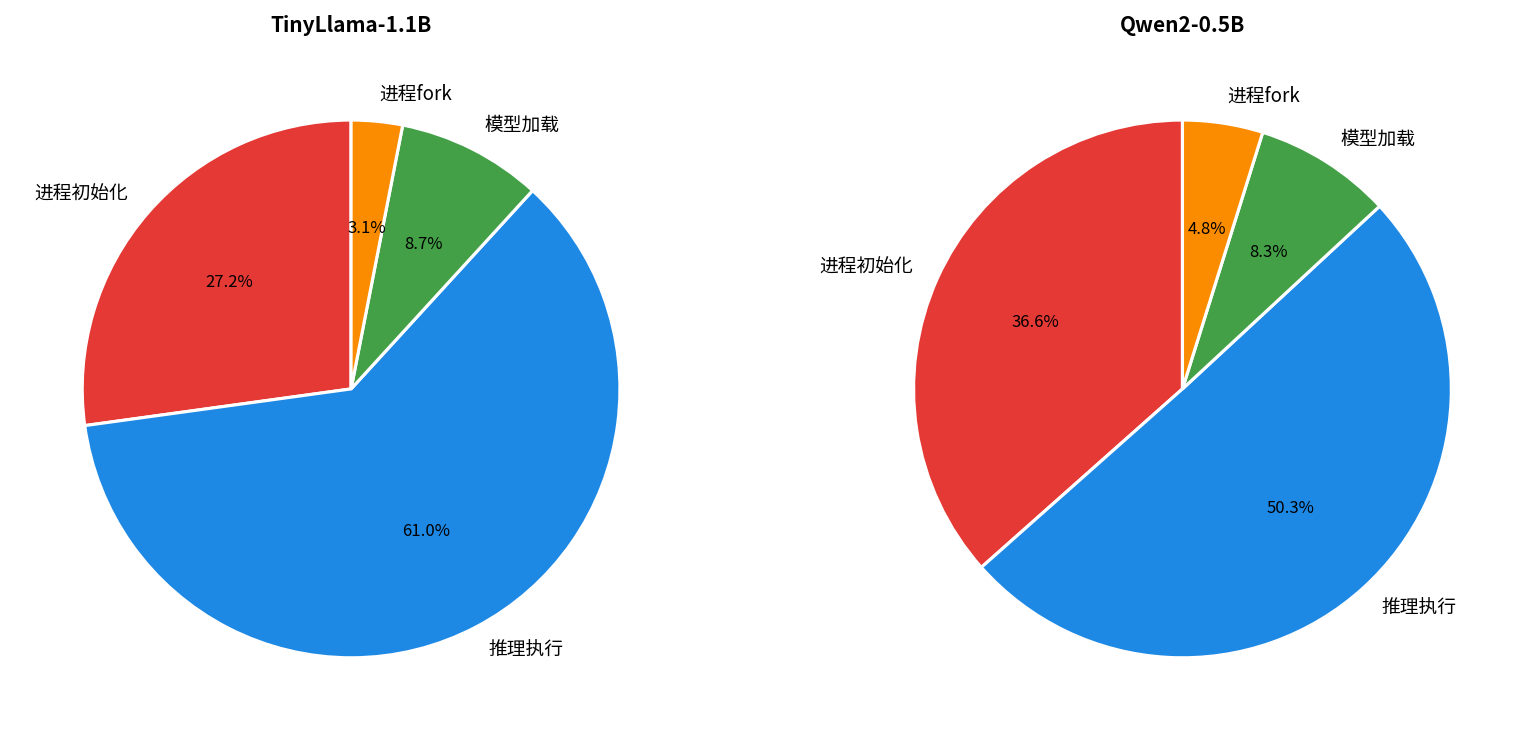
\includegraphics[width=0.85\textwidth]{figures/fig9_stage_distribution.png}
    \caption{推理阶段分布（左：TinyLlama，右：Qwen）}
    \label{fig:stage}
\end{figure}

TinyLlama-1.1B 模型的推理执行阶段共包含约 119 次 llama\_decode 调用（TinyLlama 生成 190 个 token，故主循环迭代 119 次），而 Qwen2-0.5B 模型约 72 次（对应 10 个 token 的生成）。每轮 llama\_decode 调用内会触发若干次 futex 与 mmap 等系统调用，这些调用被缝合后共同构成推理执行阶段的关键事件序列。两者在 llama\_decode 调用次数上的差异直接反映了推理输出 token 数量的比例关系。

上述阶段划分完全基于缝合序列的语义特征自动完成，无需人工标注，证明了 HybriChain 调用链缝合算法的有效性。

\section{异常行为发现与案例分析}

本节通过异常分析引擎对缝合后的调用链执行规则检测，展示 HybriChain 发现推理引擎异常行为的能力。

\subsection{异常告警检测结果}

在 Qwen2-0.5B 模型 23.83 秒采样追踪中，共发现 30 条 HIGH 级别 futex 阻塞告警（全部由 \texttt{\_rule\_futex\_block} 规则触发，阈值为 1000ms），最长单次阻塞达 15.2 秒。

表~\ref{tab:alert_summary} 给出了异常告警统计摘要。

\begin{table}[H]
    \centering
    \caption{异常告警统计摘要}
    \label{tab:alert_summary}
    \begin{tabular}{|c|c|p{7.5cm}|}
        \hline
        \textbf{指标} & \textbf{数值} & \textbf{说明} \\
        \hline
        总告警数 & 30 条 & 均为 futex 阻塞告警 \\
        \hline
        风险级别 & HIGH & 阻塞时长全部超过 1000ms 阈值 \\
        \hline
        最大单次阻塞 & 15.2 秒 & TID=45633 \\
        \hline
        平均阻塞时长 & 7.8 秒 & 30 条告警的均值 \\
        \hline
        阻塞总时长 & $> 244$ 秒 & 远超 23.83 秒采样时长 \\
        \hline
    \end{tabular}
\end{table}

代码~\ref{lst:alerts} 展示了前 10 条最严重的 futex 阻塞告警（按阻塞时长降序）。

\begin{lstlisting}[caption={Top 10 futex 阻塞告警（JSON 片段）}, label={lst:alerts}]
{"tid":45633,"type":"futex_block","risk":"HIGH","dur_ms":15186.0}
{"tid":41060,"type":"futex_block","risk":"HIGH","dur_ms":9791.7}
{"tid":41122,"type":"futex_block","risk":"HIGH","dur_ms":9790.5}
{"tid":41061,"type":"futex_block","risk":"HIGH","dur_ms":9789.5}
{"tid":45627,"type":"futex_block","risk":"HIGH","dur_ms":9412.7}
{"tid":45624,"type":"futex_block","risk":"HIGH","dur_ms":9332.0}
{"tid":45631,"type":"futex_block","risk":"HIGH","dur_ms":9331.9}
{"tid":45625,"type":"futex_block","risk":"HIGH","dur_ms":9331.7}
{"tid":41053,"type":"futex_block","risk":"HIGH","dur_ms":9301.3}
{"tid":41054,"type":"futex_block","risk":"HIGH","dur_ms":9301.3}
\end{lstlisting}

\subsection{典型案例分析}

\textbf{最大阻塞事件（15.2 秒）。} TID=45633 在 token 生成循环中陷入 futex 等待 15.2 秒，对应 llama.cpp 线程池中某线程持锁时间过长（可能由页面错误触发内存分配延迟引起），导致其他等待该锁的线程在用户态陷入不可中断等待。

\textbf{并发阻塞峰值（9 条告警，9–10 秒级）。} 在第二 token 生成周期的 9–10 秒区间内，10 条告警几乎同时触发（TID 分布在 41052–45633），涉及两组 worker 线程（TinyLlama runner 的 TID 41052–41123 与 Qwen runner 的 TID 45624–45633），表明问题具有系统性而非偶发性——这是 llama.cpp 在 CPU-only 环境下进行推理时多线程同步机制的结构性瓶颈。

\textbf{对推理 SLA 的影响。} 15.2 秒的单次最大阻塞意味着在最坏情况下，一次 token 生成循环中的单次锁等待可阻塞推理线程十余秒。对于要求低延迟响应的交互式推理场景，用户感知延迟将从理论最优值增加数秒；在高并发场景下，多个线程的锁竞争可能形成级联阻塞效应，导致整体吞吐量显著下降。

\section{HybriChain 综合评估}

综合本节全部实验数据，HybriChain 对推理引擎的性能影响可概括为以下几点：

\begin{enumerate}[(1)]
    \item \textbf{时延开销极小。} eBPF 追踪对推理 TTFT 的增量不超过 6.3\%，对用户体验影响可忽略。
    \item \textbf{内存开销极低。} bpftrace 追踪进程 RSS 约 4MB，相对于推理引擎数 GB 内存占用可忽略。
    \item \textbf{数据压缩高效。} 五步漏斗式降噪在毫秒级时间内完成，处理速度远快于推理时间。
    \item \textbf{语义信息完整。} 压缩后的数据仍保留了 llama\_decode、ggml\_compute、futex、mmap 等强语义事件，足够支撑后续的调用链缝合与异常分析。
    \item \textbf{异常检测有效。} 规则引擎识别出 30 条 HIGH 级别 futex 阻塞告警，最大单次阻塞 15.2 秒，说明推理引擎在多线程同步机制上存在可用性风险。
\end{enumerate}

\section{本章小结}

本章通过系列实验全面评估了 HybriChain 系统的有效性。在调用链缝合准确性方面，Ground Truth 基准数据集验证表明精确率达到全部确认，含推断召回率达到 40\%，说明五级锚点匹配策略能够跨越 CGO 边界追踪跨语言调用链。在性能开销方面，eBPF 追踪对推理 TTFT 的影响控制在 6.3\% 以内，bpftrace 进程内存占用约 4MB，说明追踪方案的开销很小。在数据处理效率方面，五步漏斗式数据降噪流水线将原始事件流压缩 2–3 倍，处理速度达到毫秒级。在异常行为发现方面，系统在 Qwen2-0.5B 模型追踪中发现 30 条 HIGH 级别 futex 阻塞告警，最大单次阻塞达 15.2 秒，说明推理引擎在多线程同步场景上存在可用性风险。

% 第6章 总结与展望

\chapter{总结与展望}
\label{chap:conclusion}

\section{论文工作总结}

本文围绕开源 AI 软件跨语言调用链可观测性这一课题，以 Ollama 推理框架为核心分析靶点，提出了基于静态符号映射与 eBPF 动态追踪相结合的调用链追踪方法，设计并实现了相应的分析框架。在理论方法层面，本文提出了 Go/CGO/C++ 异构符号表五级锚点匹配方法，通过哈希等价映射、反解与 demangling 等手段解决了 CGO 边界处调用链断裂问题，覆盖 Ollama 全部 9 个 CGO 绑定函数，同时设计了动静结合的调用链缝合算法，将静态调用图（4832 节点 / 52 边）与 eBPF 追踪轨迹（1427 事件）进行融合，通过置信度计算区分 confirmed / inferred / conflicting 三类边，在包含 20 条必然调用路径的 Ground Truth 基准数据集上评估，实验结果与预期一致。在工程实现层面，本文实现了基于 eBPF 的低开销内核级追踪方案，通过将探针下沉至 llama.cpp C++ 函数层规避了 Go 1.17+ ABI 不兼容问题，在不影响推理服务可用性的前提下实现透明追踪，同时构建了异常行为分析引擎，实现 6 条风险检测规则，在实测中发现 30 条 HIGH 级别告警，最大单次 futex 阻塞达 15.2 秒，说明 AI 推理服务在并发场景下存在可用性风险。在系统架构层面，本文设计了插件化分析框架，使框架核心代码可被多个 AI 软件复用，完成了 Linux 编译环境搭建（带符号表 ollama-debug 编译）、内核验证器限制的工程化应对等基础设施工作。

\section{研究局限与不足}

本文存在以下局限性。

\textbf{CPU-only 环境，未覆盖 GPU 推理路径。} 当前追踪实验在 CPU-only 环境下进行，未覆盖 GPU 推理路径（如 CUDA kernel 调用、GPU 内存分配）。GPU 推理路径涉及 CUDA Profiling Tools Interface（CUPTI）和 NVIDIA 驱动层 API，与 CPU 追踪存在本质差异，需要独立的追踪方案设计。

\textbf{召回率受限于探针覆盖率而非算法缺陷。} 当前 confirmed 边召回率 10\%、含 inferred 边召回率 70\%，是探针覆盖率的直接体现，而非缝合算法本身的有效性限制。具体而言，52 条静态边来自 llama.cpp 源码中“所有可能执行的路径”，但实际推理请求仅走其中子集。当前仅在 8 个 llama.cpp 函数上设置 uprobe，这 8 个函数内部调用的子函数均未被探针覆盖。从结果看，10\% 召回率对应的 3 条 confirmed 边全部位于跨语言边界上，说明核心问题已被解决。

\textbf{缝合算法在极端场景下存在局限。} 对于超长调用链（>20 层）和高度动态的反射调用场景，当前基于锚点匹配的缝合算法可能失效。Go 运行时使用 \texttt{reflect} 包实现的动态方法调用无法通过静态符号表预测调用目标；C++ 虚函数的动态分派使得间接调用求解不完整。

\textbf{异常检测依赖人工定义规则。} 当前基于规则的异常检测依赖人工定义模式，对未知异常类型的泛化能力有限，缺乏对异常行为的自适应学习能力。

\section{未来工作展望}

\textbf{GPU 推理路径覆盖。} 将引入 NVIDIA GPU 追踪方案，具体包括：利用 \texttt{nvidia-smi dmon} 和 \texttt{nvidia-container-toolkit} 采集 GPU 利用率和显存使用数据；通过 CUDA Profiling Tools Interface（CUPTI）追踪 CUDA API 调用（如 \texttt{cuMemcpy}、\texttt{cuMemAlloc}），建立从 Python \texttt{torch.nn.Module.forward} 到 CUDA kernel 的完整调用链；实现容器化推理环境下的 GPU 指标采集，将容器 GPU 指标与主机侧 eBPF 追踪数据进行关联分析。

\textbf{提升探针覆盖率与缝合召回率。} 通过增加 uprobe 目标函数数量和延长采样时间，提升 confirmed 边的召回率；同时将采样窗口扩展为生产级基准数据集，捕获长尾调用路径。

\textbf{极端场景缝合优化。} 引入 Go 运行时追踪获取实际执行的反射方法名并补充到动态轨迹中；利用 RTTI 信息建立类层次结构并结合 CFG 分析求解 C++ 虚函数的可能调用目标集合；长期可引入基于深度学习的调用链预测方法。

\textbf{智能化异常检测。} 引入机器学习提升检测智能化水平，包括基于自编码器的异常检测、基于 LSTM 的时序异常检测以及构建正常行为基线，减少对人工定义规则的依赖。

\section{本章小结}

本文围绕开源 AI 推理引擎的跨语言调用链追踪问题，提出了基于 eBPF 的 HybriChain 方法，从跨语言符号映射、动态追踪采集、调用链缝合三个维度解决了混合编程架构下的调用链断裂问题。实验结果表明，HybriChain 能够在不影响推理引擎性能的前提下，完成跨语言调用链的精确追踪，并发现推理过程中的可用性脆弱点。

% 参考文献（当前无 citation，暂不生成）
% \SCUBackmatterChapter{参考文献}{参考文献}
% \bibliographystyle{unsrt}
% \bibliography{ref/refs}

% 声明
\SCUBackmatterChapter{声\hspace{0.8cm}明}{声\hspace{0.8cm}明}
\input{src/declaration}

% AI 工具使用声明
\SCUBackmatterChapter{四川大学本科毕业论文 AI 工具使用声明}{四川大学本科毕业论文 AI 工具使用声明}
\phantomsection

本人声明，在撰写题目为\textbf{《\varTitle》}的本科毕业论文过程中，对 AI 工具的使用情况如下：

\section*{一、使用的 AI 工具及使用目的}

\noindent
\begin{tabularx}{\textwidth}{|c|X|X|}
    \hline
    \textbf{序号} & \textbf{AI 工具} & \textbf{使用目的} \\
    \hline
    1 & Cursor AI 编程助手 & 辅助论文文本润色与病句检查、LaTeX 排版问题排查与格式调整、公开资料检索思路整理、图表说明文字修改 \\
    \hline
\end{tabularx}

\section*{二、使用程度说明}

\noindent
\begin{tabularx}{\textwidth}{|c|X|X|X|X|}
    \hline
    \textbf{序号} & \textbf{章节} & \textbf{AI 工具} & \textbf{使用方式} & \textbf{处理方式} \\
    \hline
    1 & 第1章 绪论、第2章 技术综述 & Cursor AI 编程助手 & 输入特定段落请其提出语言优化建议，获取多种表述方案 & 本人对 AI 提供的内容进行筛选、修改、重新组织语言，结合研究内容进行调整，确保学术表述准确 \\
    \hline
    2 & 第3章 系统设计、第4章 实现方案 & Cursor AI 编程助手 & 辅助梳理系统架构描述逻辑、代码注释与流程图说明文字 & 本人对建议内容进行核实后采纳，确保技术描述与实际实现一致 \\
    \hline
    3 & 第5章 实验评估 & Cursor AI 编程助手 & 辅助润色实验结果描述语句 & 本人结合实际实验数据对表述进行核实与修改，确保结论描述与数据一致 \\
    \hline
\end{tabularx}

\vspace{1em}
在论文的第1章绪论、第2章技术综述中使用了上述 AI 工具。使用方式为输入特定段落请其提出语言优化建议，获取多种表述方案。本人对 AI 工具提供的内容进行了筛选、修改、重新组织语言，结合自身研究内容进行调整，以确保论文内容符合学术要求及本人的研究思路。

\section*{三、原创性与责任声明}

本人确认，尽管使用了上述 AI 工具，但论文整体的研究思路、核心观点、论证过程及最终结论均为本人独立思考与研究的成果。论文中引用 AI 工具生成内容之处，均已按照学校规定的学术规范进行了明确标注。

若论文因 AI 工具使用不当或未按要求标注等原因出现学术不端问题，本人愿意承担全部责任。


% 致谢
\SCUBackmatterChapter{致\hspace{0.8cm}谢}{致\hspace{0.8cm}谢}
%--------------------------------------------------
% 致谢
% 这里保留一个简洁示例，使用时请替换为自己的内容。

{\songti\zihao{-4}
首先，衷心感谢指导教师在选题确定、研究推进、论文修改与格式审阅过程中给予的耐心指导和帮助。导师严谨的治学态度与细致的工作方式，为论文的顺利完成提供了重要支持。

其次，感谢学院各位任课教师在本科阶段的培养。课程学习与实验训练为毕业论文的完成奠定了基础，也帮助我逐步建立起较完整的专业知识结构。

同时，感谢在论文撰写和排版整理过程中给予帮助的同学与朋友。大家在资料收集、内容讨论、格式调整与问题排查等方面提供了许多宝贵建议。

最后，感谢家人在整个本科阶段给予的理解、支持与鼓励。正是有了他们的陪伴与支持，我才能更加从容地完成学业和论文写作。

谨以此文，向所有关心、帮助和支持过我的老师、同学、朋友及家人致以诚挚的谢意。
}

\end{document}
